% Compile: pdflatex fixed_point_atlas.tex
% Vector figure; standalone permits \includestandalone in a parent article.
% Audited against fixed_points_mix.pdf, v0.10, sections 3--6; see audit comments below.
% -> is implication; an asterisk on an edge means the reverse fails.
% Missing edges carry no non-implication claim. Dotted arrows abbreviate schema families.
\documentclass[tikz,multi=tikzpicture,border=5mm,10pt]{standalone}
\usepackage[T1]{fontenc}
\usepackage{lmodern,amsmath,amssymb,mathtools}
\usetikzlibrary{arrows.meta,calc,positioning,backgrounds,fit}
\newcommand{\gF}{\mathsf{gFPP}}
\newcommand{\gU}{\mathsf{gU}}
\newcommand{\gUF}{\mathsf{gUFPP}}
\newcommand{\gT}{\mathsf{gTFPP}}
\newcommand{\SC}{\mathsf{SC}}
\newcommand{\FL}{\mathrm{FL\ddot ob}}
\newcommand{\Lo}{\mathrm{L\ddot ob}}
\newcommand{\sL}{\mathrm{sL\ddot ob}}
\newcommand{\strict}{\ast}
\definecolor{ink}{HTML}{161616}
\definecolor{exist}{HTML}{333333}
\definecolor{unique}{HTML}{333333}
\definecolor{term}{HTML}{333333}
\definecolor{sep}{HTML}{303030}
\tikzset{every node/.style={text=ink,font=\normalsize},
 p/.style={draw=ink!65,fill=white,align=center,inner xsep=6pt,inner ysep=5pt,minimum height=.65cm},
 e/.style={p,draw=exist!75,fill=black!2},u/.style={p,draw=unique!75,fill=black!2},t/.style={p,draw=term!75,fill=black!2},
 arr/.style={-{Stealth[length=2.4mm,width=1.6mm]},line width=.55pt,draw=ink},
 sa/.style={arr},eq/.style={Stealth-Stealth,line width=.55pt},
 lab/.style={font=\small,fill=white,inner sep=1.2pt},
 small/.style={font=\small,align=center},
 box/.style={draw=ink!23,rounded corners=2pt,line width=.4pt},
 title/.style={font=\bfseries\small,anchor=west,text=ink!85}}

\newcommand{\FC}{\mathsf{FC}}
\newcommand{\Ver}{\mathsf{Verum}}
\newcommand{\UTF}{\mathsf{UTF}}
\newcommand{\WF}{\mathsf{WFL}}
\newcommand{\Abs}{\mathsf{Abs}}
\newcommand{\Head}[2]{\node[font=\Large] at (16,.5) {#1};\node[small] at (16,-.25) {#2};}

% ----------------------------------------------------------------------
% SCOPE AND AUDIT (comments only; not printed).
% F^k/U^k/UF^k/TF^k: existence/at-most-one/unique existence/finite-parameter-
% term selections for all k-indexed finitary guarded systems. A countable
% system may use countably many parameters, but each coordinate term is finite.
% UTF^k = TF^k and U^k. Superscript <omega means all finite cardinalities.
% FPP_{u<=n}: all unary terms with <=n unguarded occurrences; no restriction
% on the number of guarded occurrences. No strictness is asserted here.
% sLoeb[Box^n] is (Box^n x -> x)<=x. All unnamed arrows are implications,
% not claims of strictness. Residual principles are specified below.
%
% New assertions beyond the supplied manuscript, checked by direct arguments:
% (1) FC_h gives UTF^k for every cardinal k. Let b_j=Box^j0. The congruence
% generated by b_j=1 is refined by the one generated by b_{j+1}=1; K,C show
% Box sends equality modulo the first to equality modulo the second. Each
% guarded iterate moves one level; at h the congruence is equality. Thus T^h
% is a constant map on A^k. Every coordinate of T^h(0) is still a finite term.
% This uses no common finite bound on row arities and no infinitary operation.
% (2) Conversely TF^omega+U^omega => FC_h for some h (no contraction needed).
% Use x_i=a_i meet Box x_{i+1}. At a_i=1 the selected solution is all 1 by
% U^omega. The finite term selecting x_0 omits some a_h, h>=1. Set only a_h=0.
% Its value stays 1, whereas the equations imply x_0<=Box^h0. Thus FC_h.
% (3) K gives Box(Box x->x) Box^2x<=Box x; hence FC_2=>FLoeb.
% More generally FC_n=>WFL_{n-1}, and applying Box^{n-2}, C and monotonicity
% gives FC_n=>D_{n-1}. Box^n is constant 1, so sLoeb[Box^n] also holds.
% (4) For strict D_n and WFL_n ladders use P_h=(Q cap[0,1])^h, with
% (Box x)_j=min({1} union {x_i:i<j}). FC_h holds, hence all UTF^k.
% P_h satisfies D_d and WFL_d iff d>=h-1. For failure use x_0=3/4,
% x_d=1/4 (WFL_d), respectively x_1=1/4 (D_d), other entries 1,
% and inspect coordinate d+1. Thus every displayed adjacent step is strict.
% (5) For strict FL+sLoeb[Box^d] use finite Boolean prefix frames of height d+1.
% Boolean sLoeb[Box^d] iff FC_d. All those Boolean frames satisfy FL.
% FL+CP does not imply sLoeb: manuscript Example 4.6. FL need not imply CP:
% a two-world irreflexive transitive Boolean frame. FL+Abs iff sLoeb: if
% r=Box a->a, Abs and FL give r=r Box r<=r Box a<=a.
% (6) FL does not imply F^omega. In the free countably generated Boolean GL
% algebra suppose x_i=q_i meet Box x_{i+1} has a solution. Its x_0 is a term
% omitting some q_h. Evaluate in a finite prefix frame of height h+1. At all
% q_i=1, FC_{h+1} forces x_0=1. Changing only q_h to 0 leaves the term x_0
% unchanged, but the equations force x_0<=Box^h0, false at the top world.
% The same algebra satisfies all finite UTF by the manuscript's FL theorem.
% (7) FL+F^omega need not imply U^omega. Take a nonprincipal ultraproduct
% of Boolean prefix algebras of heights n+1. All FL identities persist.
% Every countable system has a solution: at coordinate n solve its first n
% equations, setting unknowns of index >=n to 0; the diagonal sequences solve
% each fixed equation modulo the ultrafilter. But x_i=[Box^{max(n-i,0)}0]
% and x_i=1 are distinct solutions of x_i=Box x_{i+1}. This also separates
% every finite-system uniqueness principle from U^omega.
% (8) UF^omega does not imply TF^omega even under FL: use P(N) with strict
% prefix Box. At world m every guarded row depends only on worlds <m;
% recursion on m solves every cardinality uniquely. No FC_h holds, so (2)
% refutes TF^omega. This also witnesses strict UTF^omega=>UTF^{<omega}.
% (9) Complete lattice + Ctr_Box + Loeb gives UF^k for all k. For a system T,
% iterate interval bounds [l,u], replacing them with [inf T[l,u],sup T[l,u]],
% taking sup lower bounds/inf upper bounds at limits. This nested process
% stabilizes. Let e=meet_i(u_i->l_i). Substitution estimates and idempotence
% of Box e give Box e<=E(Tx,Ty) for all x,y in [l,u]. Distributing multiplication
% over the supremum gives Box e * sup T[l,u] <= inf T[l,u]. At stabilization
% Box e<=e, so Loeb yields e=1 and l=u. The same meet-of-equalities argument
% proves uniqueness. No arbitrary-meet preservation by Box is assumed.
% (10) Standard [0,1]_MV+CP: K makes Box 1-Lipschitz. Every finite subsystem
% has a solution by Brouwer after its external variables are assigned values;
% compactness of the product cube gives F^k for every cardinality.
% (11) Independence of SC_{2^j} even over CP+gU+SC: localize Q[eps] only at
% 1+eps and the selected pairwise coprime cyclotomic factors 1+eps^{2^j}.
% The unique SC_d solution is (eps^d+a)/(1+eps^d); its value at a=0 excludes
% every unselected factor. The infinitesimal affine estimate retains gU.

% ----------------------------------------------------------------------


% Continuity revision: ordinary, Scott, and metric continuity are kept distinct.
% Sc^up/down preserve nonempty directed suprema / filtered infima. On a complete
% chain these together are equivalent to order-topology continuity. The reverse
% Loeb=>R_omega arrow uses Sc^up and existence of the orbit supremum.
% R_omega=>Loeb uses only monotonicity. FC_<omega denotes finite attainment.
% Ordinal iteration at limits uses suprema, only in the complete-lattice panel.
% The convex-space source implies all-cardinality finitary systems by applying
% Schauder--Tychonoff to A^k. The component source only claims unary gFPP.
% The inverse-limit source uses base-algebra congruences and improvement by Box;
% its associated bounded complete prefix ultrametric has max-nonexpansive base
% operations. Thus Banach applies to A^k for every cardinal k.
% C^g_omega: each finitely satisfiable countable guarded system is satisfiable.
% L_n^omega: [(Box a_{i+1})^n<=a_i for all i] => a_0=1.
% L_var^omega permits a separately chosen finite positive exponent at each i.
% The finite-frontier error argument proves L_n^omega <=> U^omega_{<=n}, and
% L_var^omega <=> U^omega. Uniform-exponent edges are separated by affine MV
% chains q=1/(n+1); vertical edges by ultraproducts of finite Boolean GL frames.
% The weighted MV countable criterion needs a uniform margin sup_i W_q(t_i)<1.
% The antitone rows assume a bounded linear continuum, including density and
% Dedekind completeness; Box neg continuity alone on a dense subchain is not enough.
% The supplied shared discussions were retrieved directly on 2026-10-27. Their
% results were checked individually; no claim of novelty is made by this figure.

% RESIDUAL REVISION (2026-10-27); all systems below are finitary and guarded.
% e_n=Box^n 0; F_n is the multiplicative filter generated by e_n;
% theta_n relates x,y iff e_n^k <= (x->y) meet (y->x) for some positive k.
% RS_omega: intersection theta_n=Delta. RP_omega: each theta-compatible
% sequence a_n has a representative a congruent to a_n modulo theta_n.
% RC_omega=RS_omega and RP_omega, equivalently the canonical map
% eta:A -> lim_n A/theta_n is an isomorphism. These are not first-order axioms.
% R_omega means the supremum of the orbit e_n exists and is 1; this does not
% assume unrelated suprema. OC_omega means that supremum exists and Box
% preserves it. Scott continuity implies OC_omega when that supremum exists.
% Orbit idempotence: (Box0)^2=Box0 iff e_n^2=e_n for all n. Induct using
% (Box e)^2 <= Box(e^2); the reverse inequality is integrality. Under this
% identity theta_n is equality after multiplication by e_n, so RS iff R.
% With omega-chain completeness compatible approximants glue as
% a=sup_n e_n*a_n, proving RP if R holds. The two extra hypotheses in the
% corresponding printed row are CUMULATIVE, not alternative assumptions.
% NK implies Box improves theta_n agreement to theta_{n+1}. All base
% operations preserve theta_n. By simultaneous iteration on A^k, RC yields
% UF^k for EVERY cardinal k, while RS yields U^k for EVERY cardinal k.
% No uniform row arity bound, Mix, or metric is required.
% Strict chain witnesses, from left to right:
% (i) P(N) with strict-prefix Box: RC but no finite FC.
% (ii) finite/cofinite Boolean subsets of N with strict-prefix Box: RS but
% not RP (the coherent finite traces of the even integers do not glue).
% This algebra ALSO has UF^k for every k: solve in P(N) by induction on
% world height; every Box image in P(N) is a finite prefix or N, hence is
% in the finite/cofinite algebra. Guardedness forces every solution coordinate
% back into that subalgebra. Boolean prefix FL holds there as well.
% (iii) standard MV with Box x=(1+x)/2: R, all theta_n universal, not RS.
% (iv) P(omega+1) with strict predecessor Box: Loeb but not R_omega.
% RS+gTFPP need not give F^omega: take the free countably generated algebra
% of the variety generated by all finite Boolean prefix algebras. If two
% terms differ, some finite prefix valuation separates them; at its height h,
% e_h=1, hence theta_h separates them. Thus RS. All generators satisfy FL,
% hence gTFPP. The parameter-omission system described in audit (6) has no
% countable solution. This argument does not require an appeal to GL FMP.
% All-UF+sLoeb need not give RS: complete Godel chain omega+2, Box successor
% capped at the top, has sLoeb and all UF by audit (9), but R_omega fails.
% ACC collapses Loeb to finite FC because the orbit stabilizes; finite FC
% implies RC, RS and R, and each of the latter implies Loeb.
% The inverse-limit completion itself always has all UF by coordinate
% stabilization; its canonical congruences need NOT be identified with the
% kernels of the coordinate projections without an additional argument.


% CARDINAL STABILIZATION. For Q=F,U,UF,TF,UTF and every infinite kappa,
% Q^kappa iff Q^omega. Every vertex of a finitary dependency graph has a
% countable reachable closure. Well-order the vertices; add one reachable
% closure at a time to an already outgoing-closed solved set. Each new block
% is countable; its dependencies in the old set are parameters. F^omega
% solves the block. For U, a pair of global solutions restricts to the
% countable reachable closure of any coordinate, and U^omega identifies it.
% For TF use a countable-system term selector on each block, treating the
% finitely many old dependencies in any selected coordinate term as extra
% parameters, and substitute their already constructed finite original-
% parameter terms. All selected expressions remain finite, even at limits,
% since no new coordinate is created at a limit stage. Combine for UF, UTF.

% EXPANDED ATLAS AUDIT, 2026-10-27. New nodes are not automatically claimed
% inequivalent. Only asterisked arrows assert a verified reverse failure.
% gUFPP_{<=n}=E_n and L_n: existence and uniqueness over precisely the same
% at-most-n-occurrence class. Strict steps use rational MV q=1/(n+1).
% ESC is the designated SC term h(a)=Box a->a being a fixed point. FL gives
% Box h(a)=Box a by BTop, hence ESC. ESC supplies a term SC selector.
% SC^pow_{n,d} uses multiplicative n-th power, not n iterations of Box.
% E_n supplies existence, L_n supplies at-most-one by the n-occurrence estimate.
% CP_n / sL_n: put h=Box x->x. CP_n at h and FL give h^n<=Box h<=Box x,
% hence h^{n+1}<=x. For sL_n=>CP_n put y=x meet Box x; x Box y<=y,
% so x<=Box y->y and x^n<=y<=Box x. If Box x<=x then h=1, so sL_n=>Lo.
% Ctr_H makes h idempotent, so all sL_n collapse to sL under that condition.
% Mix(r,s)=>Mix(r+1,s+1) is substitution x:=Box x. Under 4 the second
% factor increases with its positive modal exponent, proving the horizontal
% weakening. Abs entails CP and Mix; Lo+Abs=>FL+Abs=>sL. No unsupported
% first-index monotonicity or reverse comparison is drawn.
% DG_n uses r(v)=v^n; DG gives guarded identity r(Box x); GI lets one replace
% EVERY unknown occurrence in an arbitrary system by its guarded identity.
% GI contradicts gU on a nontrivial algebra, since every element fixes e.
% DG_n+Ctr_Box gives Box x=x; Lo then forces triviality.
% AI_r is the prior MV interpolation scheme, equivalently the printed product
% normal form: B arbitrary MV algebra and Gamma(G,u) a divisible MV chain;
% the second factor may be trivial. Original e=(Box0)^r satisfies
% e vee neg e=1, Box0=e vee (neg Box0)^{oplus(r-1)}, (Box x)^r=e vee x.
% PI uses Boolean e=Box0, Box x=e vee x and divisible chain [0,neg e].
% SR=AI_2. In the nontrivial chain component L_n holds exactly for n<r:
% (Box x)^n=max(0, ((r-n)u+nx)/r). L_r fails at (1,0).
% SC's unique chain solution under AI_r is (u+r*a)/(r+1); its slope
% r/(r+1) is not in Z[1/r]. Every parameter term has finitely many affine
% slopes in Z[1/r], so SC^term is impossible on a nontrivial divisible
% component. For PI replace this by slope 1/2 versus integral term slopes.
% Restricting the parameter to rational multiples of u suffices, even in a
% non-Archimedean chain. Thus AI_r+SC^term and PI+SC^term force Verum.
% AI_r antichain and failed FPP use 2 times rational MV; failed gU uses
% the r-occurrence identity on the chain. FL and Mix failure are direct
% computations at zero. AI_r+L_n for n<r is automatic, not a new assumption.
% Divisible MV chains have base-language FPP because scalar MV polynomials
% are continuous finite piecewise integral-affine. Conversely, for a>0 and
% n>=2, the term (x -> neg a)^{n-1} has unique fixed point
% x=1-(n-1)a/n in the ambient ordered group. The branch x<=neg a would
% force x=1 and is impossible. Thus a minus neg x=a/n belongs to A.
% This gives exact group division also for a=1; a=0 is trivial.
% Finite continuous rational-affine systems over divisible ordered groups:
% translate their finite pieces into ordered-Q-vector-space formulas. Brouwer
% proves the universally parameterized existence sentence over R. Quantifier
% elimination / completeness of nontrivial divisible ordered abelian groups
% transfers the sentence to G. The bounded cube uses the named positive u;
% no Archimedean assumption is required. Continuity here includes matching
% values on all adjacent piece boundaries. No countable unguarded extension
% is claimed. Unguarded TFPP fails for Q-MV with Verum: every closed modal
% term is 0 or 1, while negation's fixed point is 1/2.
% FC_h iff every guarded h-th iterate is constant: forward by the residual
% filtration, reverse by choosing T=Box and using Box^h1=1.
% Canonical d_Box(x,y)=2^{-sup{n:x theta_n y}}, with 2^{-infty}=0.
% It is always a bounded pseudoultrametric; RS is separation. RP is Cauchy
% completeness (in the pseudometric sense). Both directions use a compatible
% representative sequence / a Cauchy subsequence with stage-n agreement.
% RC gives a complete ultrametric and Banach iteration on arbitrary powers.
% Strict Sc^up=>omegaSc^up: complete Godel chain omega_1+1 with Box x=0
% below the top and Box top=top. Every countable ascending sequence is
% preserved; the directed set of all countable ordinals is not. NK4 holds.
% Strict omegaSc^up=>OC: standard Godel chain, Box x=0 for x<1/2 and
% Box x=1 for x>=1/2. Its zero orbit is fixed, but the jump refutes omegaSc.
% OC includes existence of the orbit supremum; on the row where that supremum
% is assumed, OC+Lo iff R. R itself implies OC under N, since Box1=1.
% On complete chains interval, Lawson and order topologies coincide, and
% simultaneous directed-join and filtered-meet preservation is order continuity.
% agFPP_d is termwise arbitrarily small displacement. Actual implies
% approximate, compactness plus continuous term maps supplies the reverse.
% Dyadic affine MV is dense in its real completion, so has approximate FPP
% for all continuous term maps; SC fails because its zero solution is 1/3.
% Sol_{Par+Bek}: a chosen solution map for every finite guarded system,
% commuting with parameter substitutions and satisfying the displayed Bekic
% identity. TSol requires every coordinate selector to be a parameter term.
% Under finite uniqueness these laws follow by verifying both sides solve the
% same system. No existence-only converse to coherent choice is claimed.
% Guarded-envelope transfer: if A<=B and Box B subset A, every guarded term
% on B-valued unknowns and A-valued parameters takes values in A, by replacing
% its outermost Box subterms by elements of A. Hence every B-solution lies
% in A. Unique solvability descends as well. This proves the FinCof example.
% J^vee_k=>J^vee_{k+1}: group the last two variables in the k-ary instance;
% every resulting join omits at least one of the original variables.
% Strictness uses H_n, upsets of a root with n incomparable maximal points,
% Box U=U union Max(P minus U). This has NK4 CP sL. J^vee_k fails exactly
% when the n maximal points admit a cover by k sets with every set essential,
% i.e. k<=n. It is unrelated to the Jeroslow principle denoted J.


% COUPLED SC / CYCLE GUARDS. R is row-finite with nonnegative integer
% coefficients; d_ij is positive on nonzero coefficients. SCsys quantifies
% every parameter tuple and asks for the simultaneous displayed solution.
% The n-row uniqueness statements are restrictions of the proved full
% system uniqueness principles, and are NOT asserted as converses.
% In a finite system whose unguarded occurrence graph is acyclic, substitute
% defining terms along unguarded dependencies in reverse topological order.
% The resulting finite terms are fully guarded. Solution sets agree: in the
% reverse direction induct on the same acyclic graph to undo substitution.
% Hence existence, uniqueness and uniform term selection agree with their
% fully guarded counterparts. For infinite systems require finite reachable
% unguarded closure at each coordinate (fr_0), so the same substitutions
% remain finite per coordinate. Acyclicity alone allows p_i=p_{i+1}, which
% has distinct constant solutions on every nontrivial algebra.
% Coherent selection on page 8 is defined on the finite guarded elimination
% closure: maps obtained from finite guarded term systems by finitely many
% eliminations are admitted as inputs to the solution operator. Under unique
% finite solvability every such map is represented by a flattened finite term
% system and has a unique solution. This closes the displayed Bekic law's
% typing gap when intermediate h is not initially a term operation.
% Standard reference for the guarded Conway setting (comparison, not an
% identification with an unconstructed categorical RAMS model):
% S. Milius and T. Litak, Guard Your Daggers and Traces: Properties of
% Guarded (Co-)recursion, Fundamenta Informaticae 150 (2017), 407--449,
% doi:10.3233/FI-2017-1475, arXiv:1603.05214.
% Finite rational-affine transfer uses the classical quantifier elimination
% of nontrivial divisible ordered abelian groups. A reference is D. Marker,
% Model Theory: An Introduction, GTM 217, Springer (2002), ordered groups.
% No source-level verification here is proof-assistant certification, and
% no literature priority claim is made for the supplementary implications.

\begin{document}
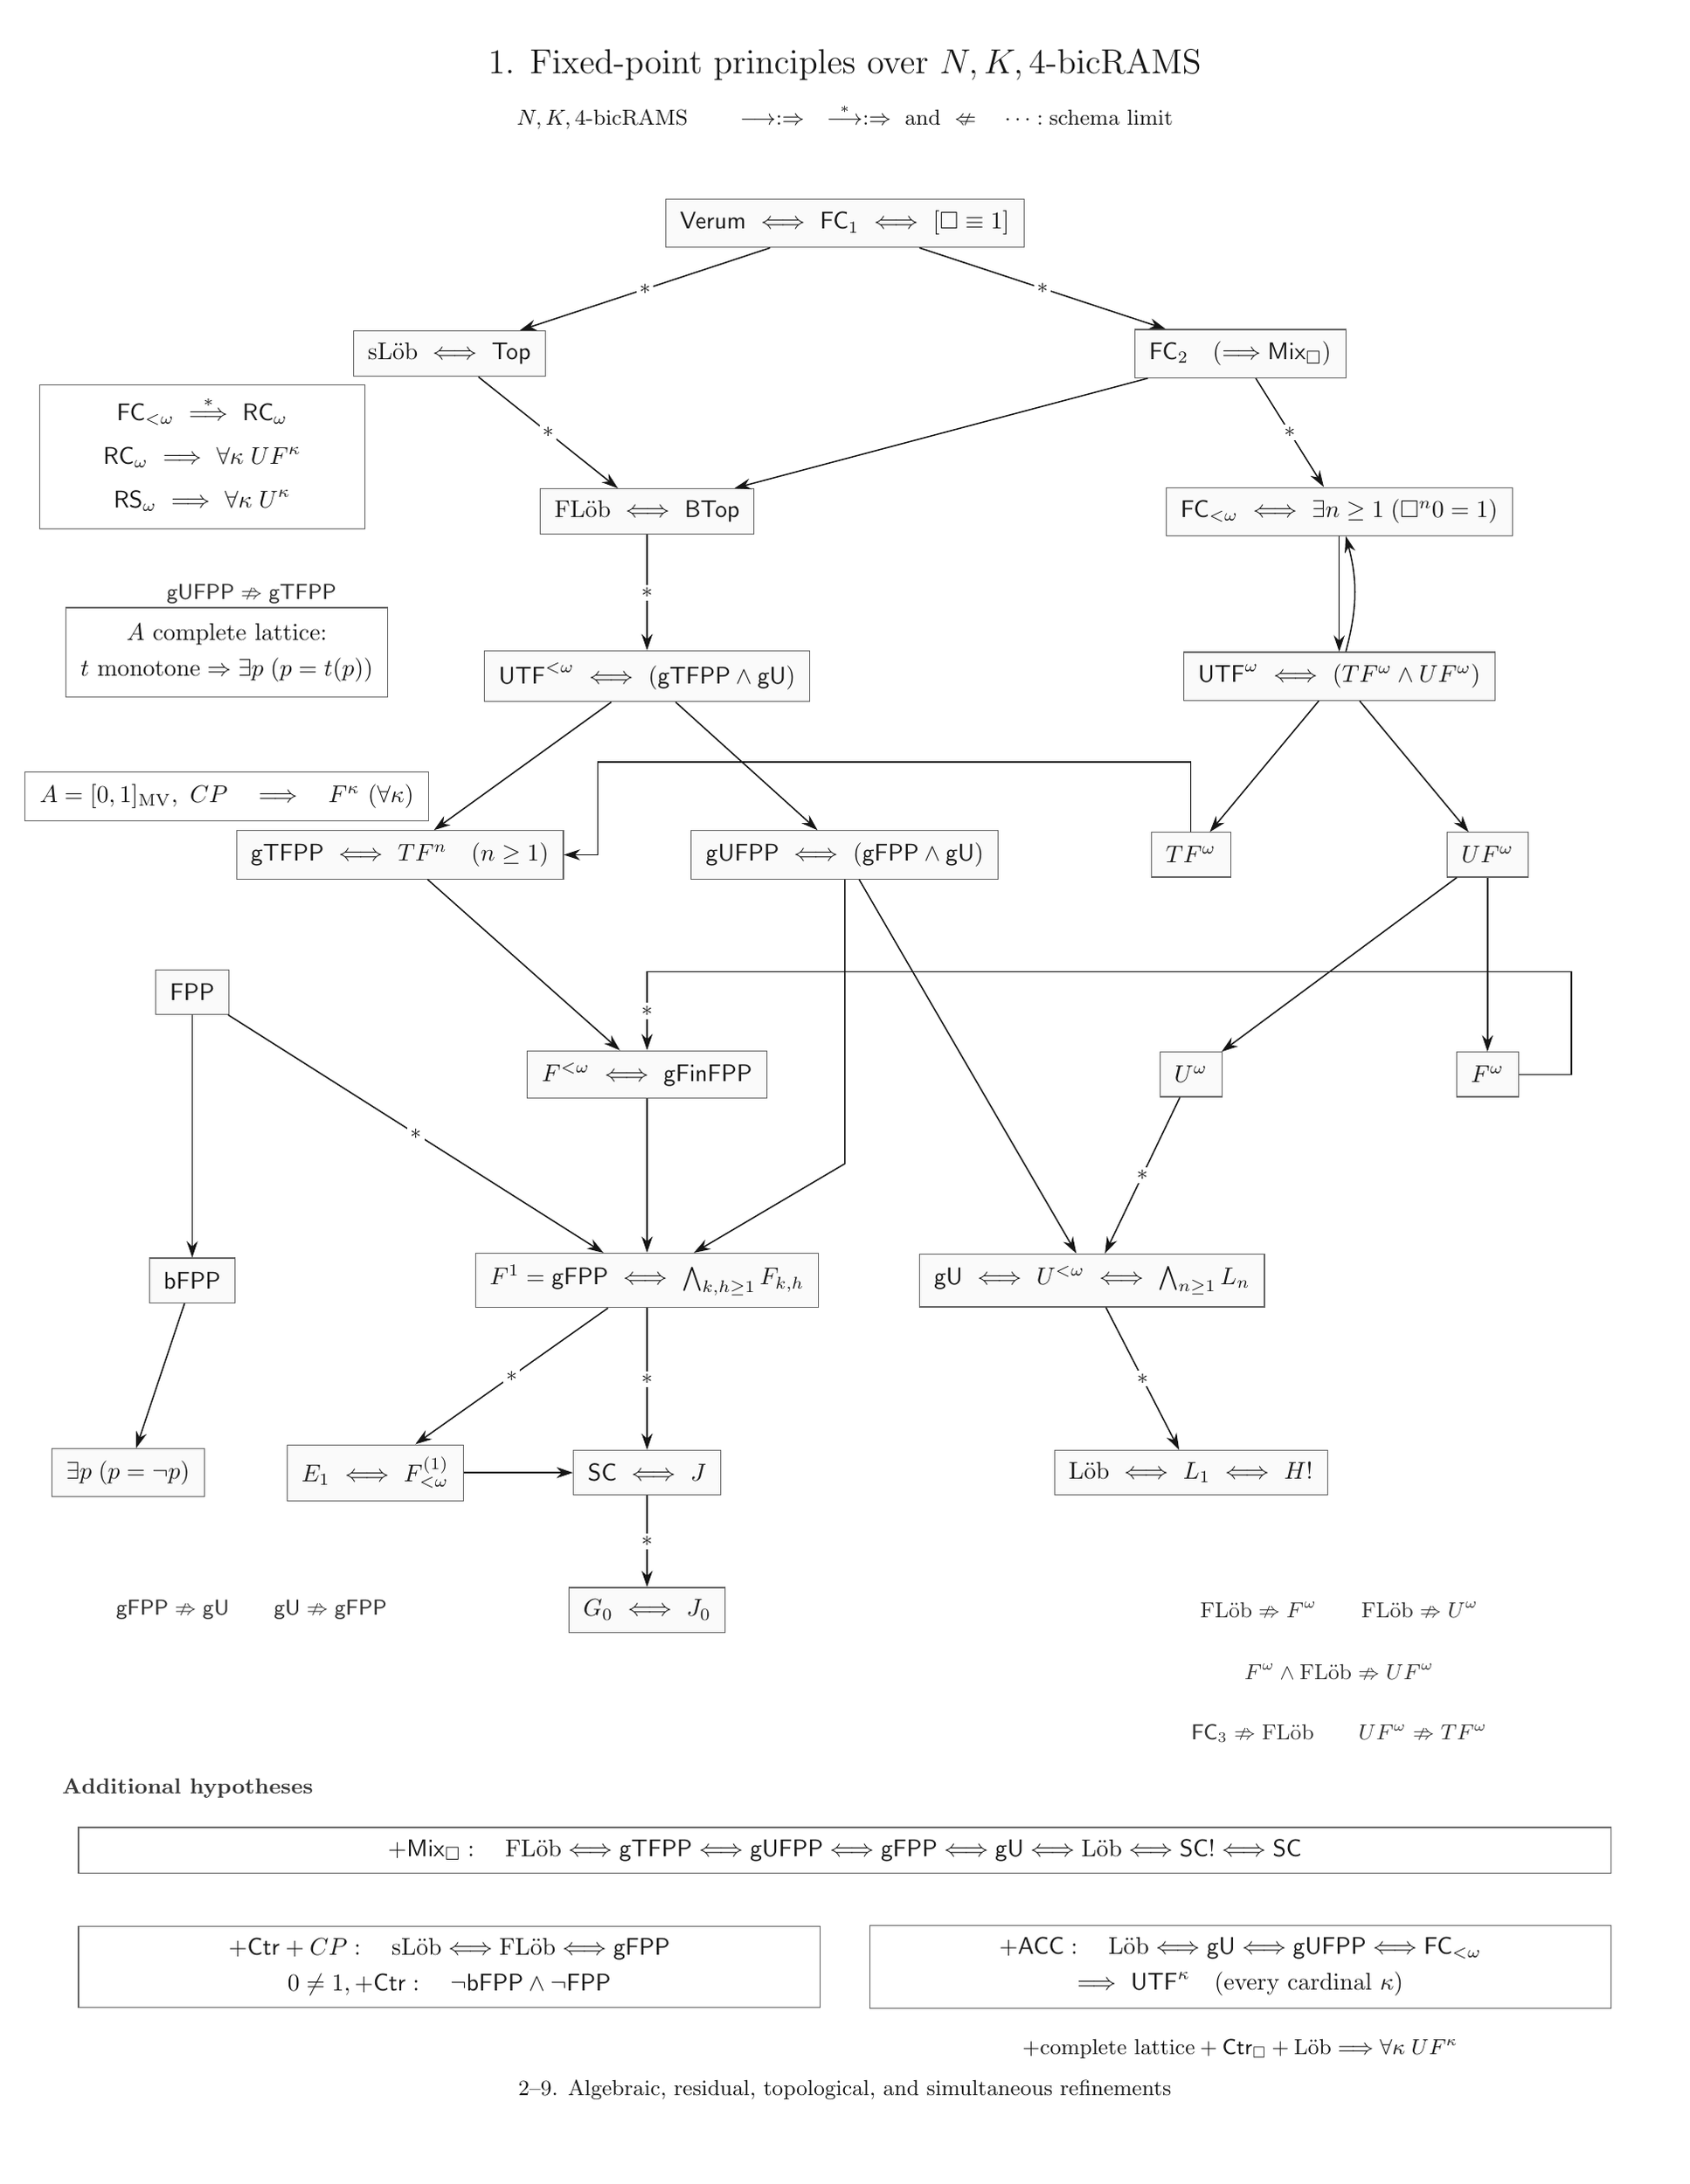
\begin{tikzpicture}[x=.72cm,y=1cm]
\path[use as bounding box] (-.6,-30) rectangle (32.6,1.1);
\Head{1. Fixed-point principles over $N,K,4$-bicRAMS}{$N,K,4$-bicRAMS $\qquad \longrightarrow:\Rightarrow\quad \overset{\ast}{\longrightarrow}:\Rightarrow\text{ and }\nLeftarrow\quad \cdots:\text{schema limit}$}
\node[t] (v) at (16,-1.8) {$\Ver\ \Longleftrightarrow\ \FC_1\ \Longleftrightarrow\ [\Box\equiv1]$};
\node[t] (sl) at (8,-3.7) {$\sL\ \Longleftrightarrow\ \mathsf{Top}$};
\node[t] (fc2) at (24,-3.7) {$\FC_2\quad(\Longrightarrow\mathsf{Mix}_{\Box})$};
\draw[arr] (v) --node[lab]{$\ast$} (sl);
\draw[arr] (v) --node[lab]{$\ast$} (fc2);
\node[t] (fl) at (12,-6) {$\FL\ \Longleftrightarrow\ \mathsf{BTop}$};
\draw[arr] (sl) --node[lab]{$\ast$} (fl);
\draw[arr] (fc2) -- (fl);
\node[t] (fc) at (26,-6) {$\FC_{<\omega}\ \Longleftrightarrow\ \exists n\ge1\;(\Box^n0=1)$};
\draw[arr] (fc2) --node[lab]{$\ast$} (fc);
\node[t] (ut) at (12,-8.4) {$\UTF^{<\omega}\ \Longleftrightarrow\ (\gT\wedge\gU)$};
\draw[arr] (fl) --node[lab]{$\ast$} (ut);
\node[t] (uwt) at (26,-8.4) {$\UTF^\omega\ \Longleftrightarrow\ (TF^\omega\wedge UF^\omega)$};
\draw[arr] (fc) -- (uwt);
\draw[arr] (uwt) to[bend right=15] (fc);
\node[t] (gt) at (7,-11) {$\gT\ \Longleftrightarrow\ TF^n\quad(n\ge1)$};
\node[u] (guf) at (16,-11) {$\gUF\ \Longleftrightarrow\ (\gF\wedge\gU)$};
\draw[arr] (ut) -- (gt);
\draw[arr] (ut) -- (guf);
\node[t] (tw) at (23,-11) {$TF^\omega$};
\node[u] (ufw) at (29,-11) {$UF^\omega$};
\draw[arr] (uwt) -- (tw);
\draw[arr] (uwt) -- (ufw);
\draw[arr] (tw) -- (23,-9.65) -- (11,-9.65) -- (11,-11) -- (gt.east);
\node[e] (ff) at (12,-14.2) {$F^{<\omega}\ \Longleftrightarrow\ \mathsf{gFinFPP}$};
\draw[arr] (gt) -- (ff);
\node[e] (fw) at (29,-14.2) {$F^\omega$};
\node[u] (uomega) at (23,-14.2) {$U^\omega$};
\draw[arr] (ufw) -- (fw);
\draw[arr] (ufw) -- (uomega);
\draw[arr] (fw) -- (30.7,-14.2) -- (30.7,-12.7) -- (12,-12.7) --node[lab]{$\ast$} (ff);
\node[e] (gf) at (12,-17.2) {$F^1=\gF\ \Longleftrightarrow\ \bigwedge_{k,h\ge1}F_{k,h}$};
\draw[arr] (ff) -- (gf);
\draw[arr] (guf) -- (16,-15.5) -- (gf);
\node[u] (gu) at (21,-17.2) {$\gU\ \Longleftrightarrow\ U^{<\omega}\ \Longleftrightarrow\ \bigwedge_{n\ge1}L_n$};
\draw[arr] (guf) -- (gu);
\draw[arr] (uomega) --node[lab]{$\ast$} (gu);
\node[e] (fpp) at (2.8,-13) {$\mathsf{FPP}$};
\node[e] (bpp) at (2.8,-17.2) {$\mathsf{bFPP}$};
\draw[arr] (fpp) -- (bpp);
\draw[arr] (fpp) --node[lab]{$\ast$} (gf);
\node[e] (sc) at (12,-20) {$\SC\ \Longleftrightarrow\ J$};
\draw[arr] (gf) --node[lab]{$\ast$} (sc);
\node[u] (lo) at (23,-20) {$\Lo\ \Longleftrightarrow\ L_1\ \Longleftrightarrow\ H!$};
\draw[arr] (gu) --node[lab]{$\ast$} (lo);
\node[e] (g0) at (12,-22) {$G_0\ \Longleftrightarrow\ J_0$};
\draw[arr] (sc) --node[lab]{$\ast$} (g0);
\node[e] (e1) at (6.5,-20) {$E_1\ \Longleftrightarrow\ F^{(1)}_{<\omega}$};
\draw[arr] (gf) --node[lab]{$\ast$} (e1);
\draw[arr] (e1) -- (sc);
\node[e] (neg) at (1.5,-20) {$\exists p\;(p=\neg p)$};
\draw[arr] (bpp) -- (neg);

\node[p,text width=4.32cm] at (3,-5.2) {$\begin{gathered}
\FC_{<\omega}\ \overset{\ast}{\Longrightarrow}\ \mathsf{RC}_\omega\\[3pt]
\mathsf{RC}_\omega\ \Longrightarrow\ \forall\kappa\;UF^\kappa\\[3pt]
\mathsf{RS}_\omega\ \Longrightarrow\ \forall\kappa\;U^\kappa
\end{gathered}$};
\node[small,text=sep] at (4,-7.2) {$\gUF\nRightarrow\gT$};
\node[p] (mvcond) at (3.5,-10.15) {$A=[0,1]_{\mathrm{MV}},\ CP\quad\Longrightarrow\quad F^\kappa\ (\forall\kappa)$};
\node[p] at (3.5,-8.05) {$\begin{gathered}A\text{ complete lattice:}\\ t\text{ monotone}\Rightarrow\exists p\;(p=t(p))\end{gathered}$};
\node[small,text=sep] at (4,-22) {$\gF\nRightarrow\gU\qquad\gU\nRightarrow\gF$};
\node[small,text=sep] at (26,-22) {$\FL\nRightarrow F^\omega\qquad\FL\nRightarrow U^\omega$};
\node[small,text=sep] at (26,-22.9) {$F^\omega\wedge\FL\nRightarrow UF^\omega$};
\node[small,text=sep] at (26,-23.8) {$\FC_3\nRightarrow\FL\qquad UF^\omega\nRightarrow TF^\omega$};
\node[title] at (0,-24.6) {Additional hypotheses};
\node[p,minimum width=22.32cm] (mixcollapse) at (16,-25.5) {$+\mathsf{Mix}_{\Box}:\quad\FL\Longleftrightarrow\gT\Longleftrightarrow\gUF\Longleftrightarrow\gF\Longleftrightarrow\gU\Longleftrightarrow\Lo\Longleftrightarrow\SC!\Longleftrightarrow\SC$};
\node[p,minimum width=10.8cm] (heyt) at (8,-27.2) {$+\mathsf{Ctr}+CP:\quad\sL\Longleftrightarrow\FL\Longleftrightarrow\gF$\\[3pt]$0\ne1,+\mathsf{Ctr}:\quad\neg\mathsf{bFPP}\wedge\neg\mathsf{FPP}$};
\node[p,minimum width=10.8cm] (acc) at (24,-27.2) {$+\mathsf{ACC}:\quad\Lo\Longleftrightarrow\gU\Longleftrightarrow\gUF\Longleftrightarrow\FC_{<\omega}$\\[3pt]$\Longrightarrow\ \UTF^\kappa\quad(\text{every cardinal }\kappa)$};
\node[small] at (16,-29) {$\text{2--9. Algebraic, residual, topological, and simultaneous refinements}$};

\node[small] at (24,-28.4) {$+\text{complete lattice}+\mathsf{Ctr}_{\Box}+\Lo\Longrightarrow\forall\kappa\;UF^\kappa$};



\end{tikzpicture}
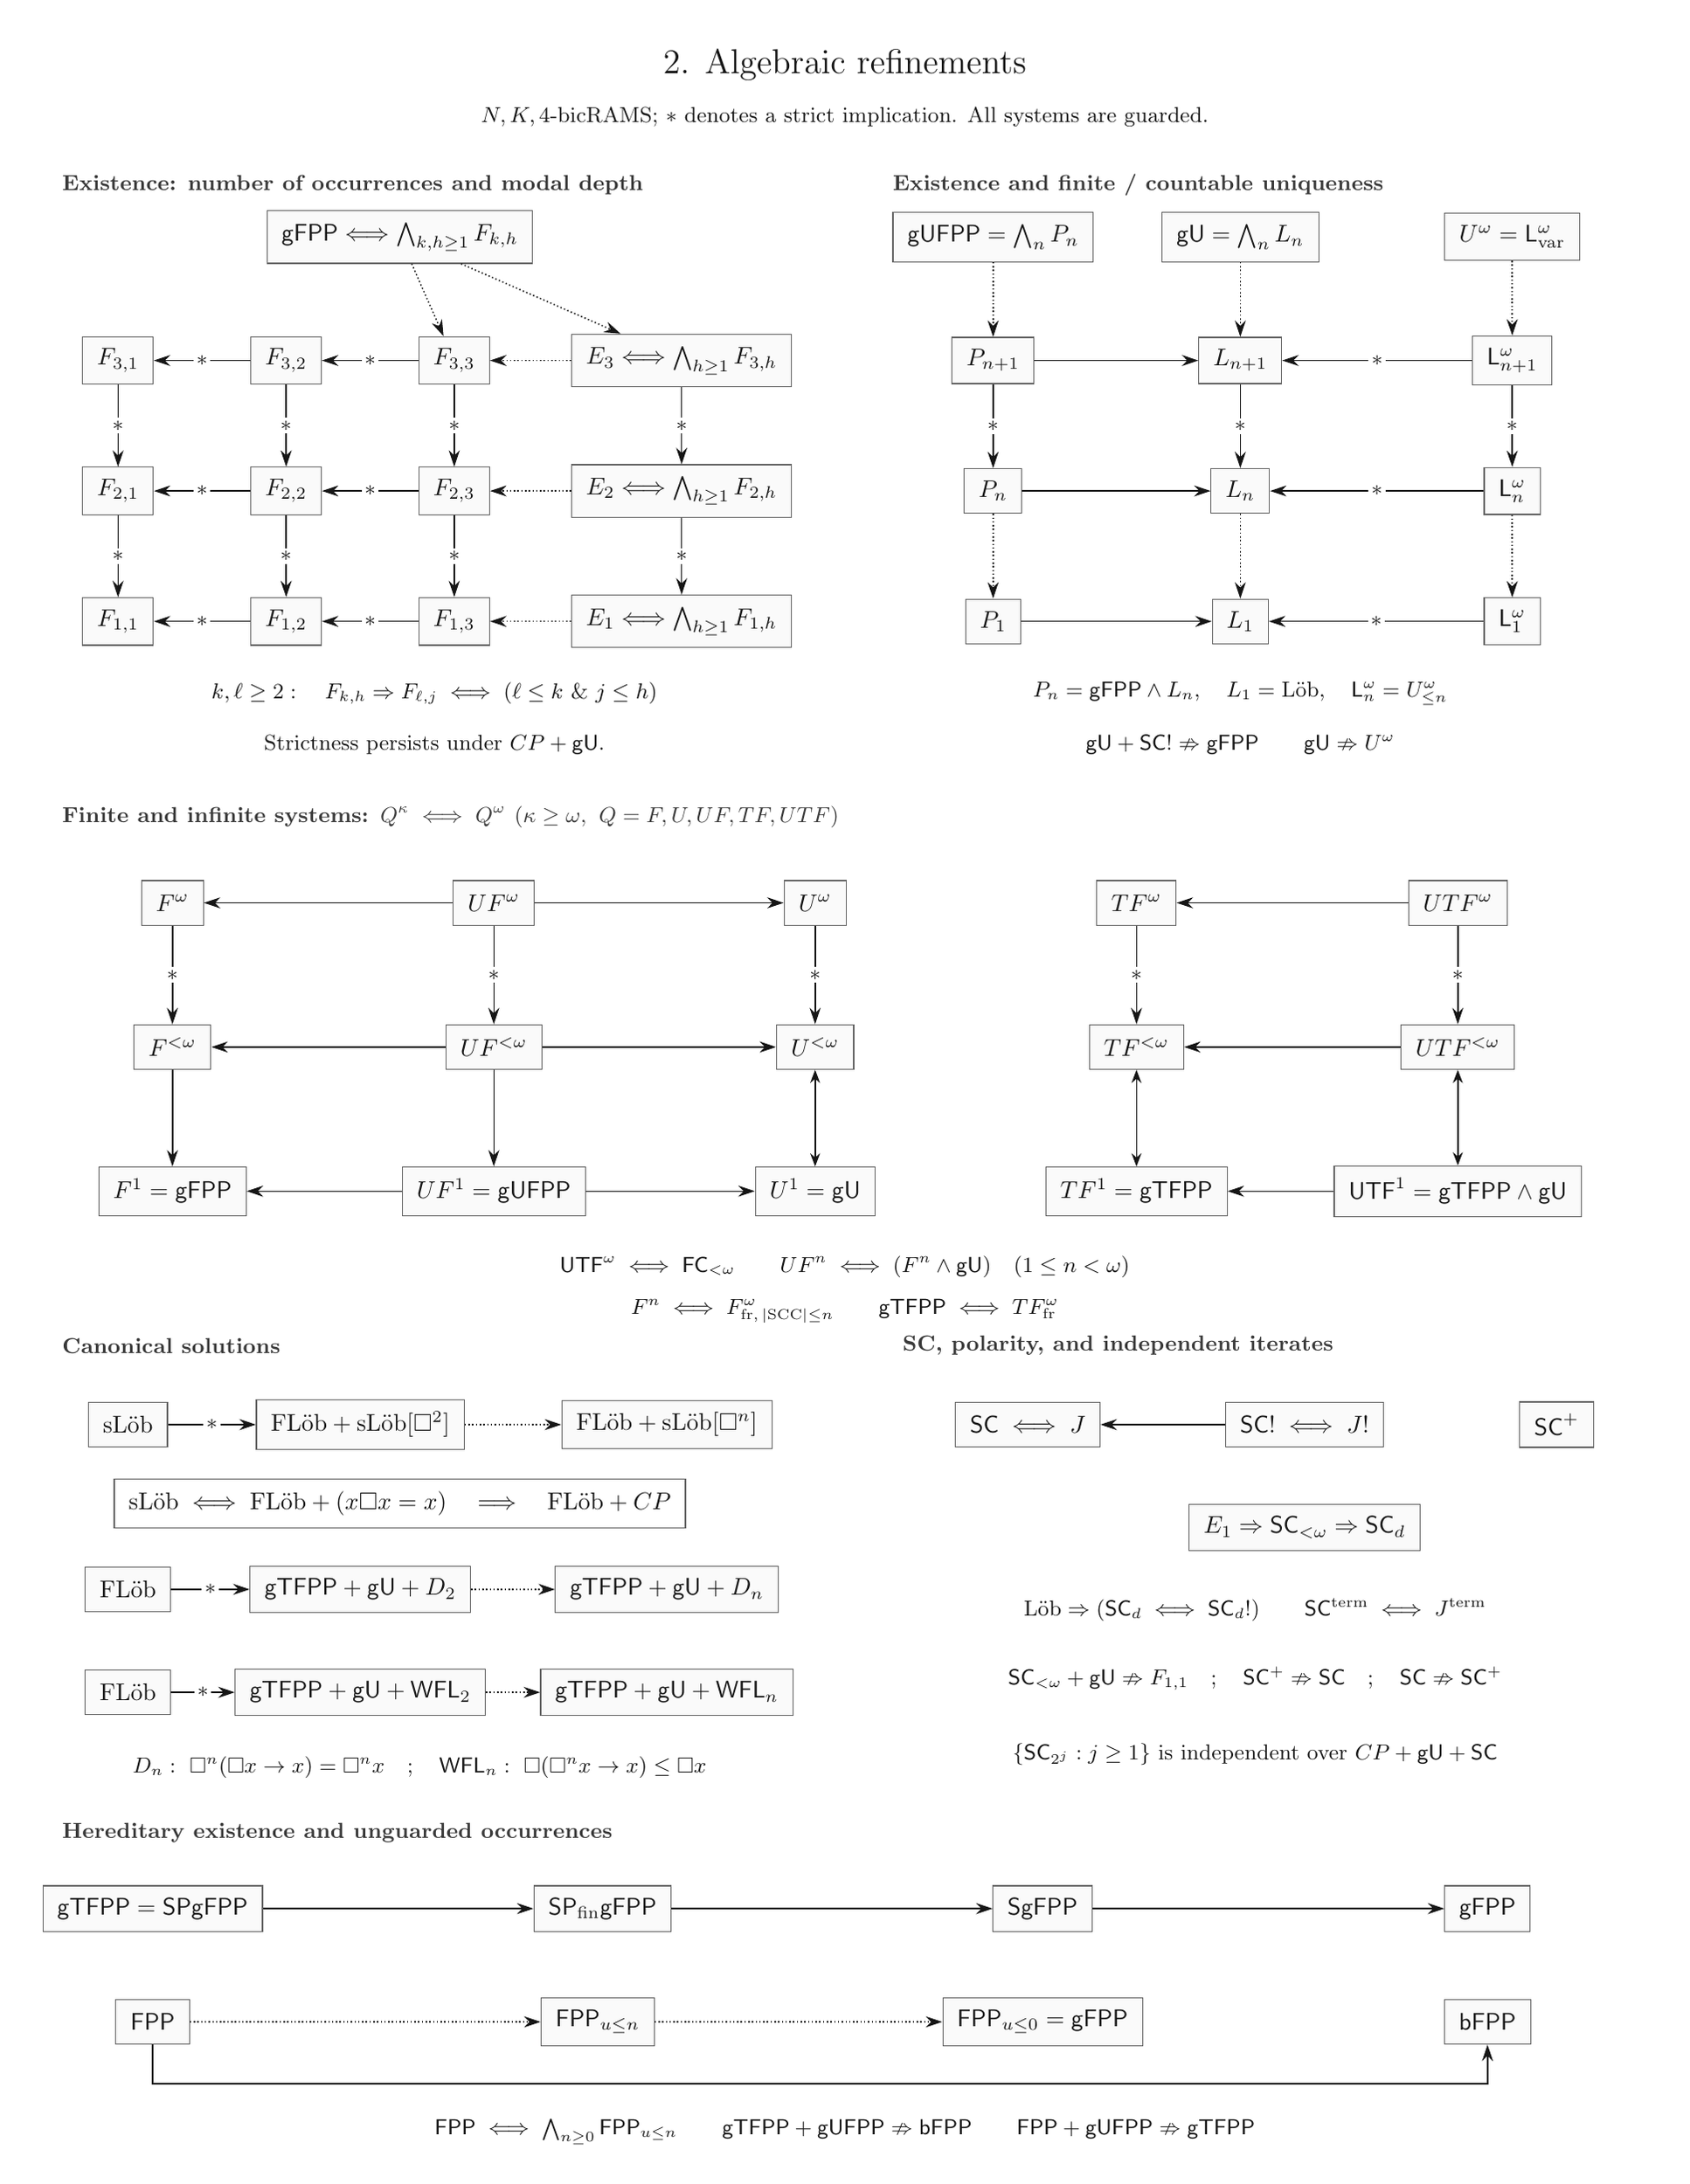
\begin{tikzpicture}[x=.72cm,y=1cm]
\path[use as bounding box] (-.6,-30) rectangle (32.6,1.1);
\Head{2. Algebraic refinements}{$N,K,4$-bicRAMS; $\ast$ denotes a strict implication. All systems are guarded.}
\node[title] at (0,-1.25) {Existence: number of occurrences and modal depth};
\node[e] (f11) at (1.3,-7.6) {$F_{1,1}$};
\node[e] (f12) at (4.7,-7.6) {$F_{1,2}$};
\node[e] (f13) at (8.1,-7.6) {$F_{1,3}$};
\node[e] (e1) at (12.7,-7.6) {$E_1\Longleftrightarrow\bigwedge_{h\ge1}F_{1,h}$};
\draw[arr] (f12) --node[lab]{$\ast$} (f11);
\draw[arr] (f13) --node[lab]{$\ast$} (f12);
\draw[arr,densely dotted] (e1) -- (f13);
\node[e] (f21) at (1.3,-5.7) {$F_{2,1}$};
\node[e] (f22) at (4.7,-5.7) {$F_{2,2}$};
\node[e] (f23) at (8.1,-5.7) {$F_{2,3}$};
\node[e] (e2) at (12.7,-5.7) {$E_2\Longleftrightarrow\bigwedge_{h\ge1}F_{2,h}$};
\draw[arr] (f22) --node[lab]{$\ast$} (f21);
\draw[arr] (f23) --node[lab]{$\ast$} (f22);
\draw[arr,densely dotted] (e2) -- (f23);
\node[e] (f31) at (1.3,-3.8) {$F_{3,1}$};
\node[e] (f32) at (4.7,-3.8) {$F_{3,2}$};
\node[e] (f33) at (8.1,-3.8) {$F_{3,3}$};
\node[e] (e3) at (12.7,-3.8) {$E_3\Longleftrightarrow\bigwedge_{h\ge1}F_{3,h}$};
\draw[arr] (f32) --node[lab]{$\ast$} (f31);
\draw[arr] (f33) --node[lab]{$\ast$} (f32);
\draw[arr,densely dotted] (e3) -- (f33);
\draw[arr] (f21) --node[lab]{$\ast$} (f11);
\draw[arr] (f22) --node[lab]{$\ast$} (f12);
\draw[arr] (f23) --node[lab]{$\ast$} (f13);
\draw[arr] (e2) --node[lab]{$\ast$} (e1);
\draw[arr] (f31) --node[lab]{$\ast$} (f21);
\draw[arr] (f32) --node[lab]{$\ast$} (f22);
\draw[arr] (f33) --node[lab]{$\ast$} (f23);
\draw[arr] (e3) --node[lab]{$\ast$} (e2);
\node[e] (gf) at (7,-2) {$\gF\Longleftrightarrow\bigwedge_{k,h\ge1}F_{k,h}$};
\draw[arr,densely dotted] (gf) -- (f33);
\draw[arr,densely dotted] (gf) -- (e3);
\node[small] at (7.7,-8.65) {$k,\ell\ge2:\quad F_{k,h}\Rightarrow F_{\ell,j}\iff(\ell\le k\ \&\ j\le h)$};
\node[small] at (7.7,-9.4) {$\text{Strictness persists under }CP+\gU.$};
\node[title] at (16.8,-1.25) {Existence and finite / countable uniqueness};
\node[u] (uf) at (19,-2) {$\gUF=\bigwedge_nP_n$};
\node[u] (gu) at (24,-2) {$\gU=\bigwedge_nL_n$};
\node[u] (uw) at (29.5,-2) {$U^\omega=\mathsf L^\omega_{\rm var}$};
\node[u] (pn+1) at (19,-3.8) {$P_{n+1}$};
\node[u] (ln+1) at (24,-3.8) {$L_{n+1}$};
\node[u] (wn+1) at (29.5,-3.8) {$\mathsf L^{\omega}_{n+1}$};
\draw[arr] (pn+1) -- (ln+1);
\draw[arr] (wn+1) --node[lab]{$\ast$} (ln+1);
\node[u] (pn) at (19,-5.7) {$P_{n}$};
\node[u] (ln) at (24,-5.7) {$L_{n}$};
\node[u] (wn) at (29.5,-5.7) {$\mathsf L^{\omega}_{n}$};
\draw[arr] (pn) -- (ln);
\draw[arr] (wn) --node[lab]{$\ast$} (ln);
\node[u] (p1) at (19,-7.6) {$P_{1}$};
\node[u] (l1) at (24,-7.6) {$L_{1}$};
\node[u] (w1) at (29.5,-7.6) {$\mathsf L^{\omega}_{1}$};
\draw[arr] (p1) -- (l1);
\draw[arr] (w1) --node[lab]{$\ast$} (l1);
\draw[arr,densely dotted] (uf) -- (pn+1);
\draw[arr] (pn+1) --node[lab]{$\ast$} (pn);
\draw[arr,densely dotted] (pn) -- (p1);
\draw[arr,densely dotted] (gu) -- (ln+1);
\draw[arr] (ln+1) --node[lab]{$\ast$} (ln);
\draw[arr,densely dotted] (ln) -- (l1);
\draw[arr,densely dotted] (uw) -- (wn+1);
\draw[arr] (wn+1) --node[lab]{$\ast$} (wn);
\draw[arr,densely dotted] (wn) -- (w1);
\node[small] at (24,-8.65) {$P_n=\gF\wedge L_n,\quad L_1=\Lo,\quad\mathsf L_n^\omega=U^\omega_{\le n}$};
\node[small] at (24,-9.4) {$\gU+\SC!\nRightarrow\gF\qquad\gU\nRightarrow U^\omega$};
\node[title] at (0,-10.45) {Finite and infinite systems: $Q^\kappa\iff Q^\omega\ (\kappa\ge\omega,\ Q=F,U,UF,TF,UTF)$};
\node[e] (Fo) at (2.4,-11.7) {$F^\omega$};
\node[e] (Ff) at (2.4,-13.8) {$F^{<\omega}$};
\draw[arr] (Fo) --node[lab]{$\ast$} (Ff);
\node[e] (F1) at (2.4,-15.9) {$F^1=\gF$};
\draw[arr] (Ff) -- (F1);
\node[u] (UFo) at (8.9,-11.7) {$UF^\omega$};
\node[u] (UFf) at (8.9,-13.8) {$UF^{<\omega}$};
\draw[arr] (UFo) --node[lab]{$\ast$} (UFf);
\node[u] (UF1) at (8.9,-15.9) {$UF^1=\gUF$};
\draw[arr] (UFf) -- (UF1);
\node[u] (Uo) at (15.4,-11.7) {$U^\omega$};
\node[u] (Uf) at (15.4,-13.8) {$U^{<\omega}$};
\draw[arr] (Uo) --node[lab]{$\ast$} (Uf);
\node[u] (U1) at (15.4,-15.9) {$U^1=\gU$};
\draw[arr,eq] (Uf) -- (U1);
\node[t] (TFo) at (21.9,-11.7) {$TF^\omega$};
\node[t] (TFf) at (21.9,-13.8) {$TF^{<\omega}$};
\draw[arr] (TFo) --node[lab]{$\ast$} (TFf);
\node[t] (TF1) at (21.9,-15.9) {$TF^1=\gT$};
\draw[arr,eq] (TFf) -- (TF1);
\node[t] (UTFo) at (28.4,-11.7) {$UTF^\omega$};
\node[t] (UTFf) at (28.4,-13.8) {$UTF^{<\omega}$};
\draw[arr] (UTFo) --node[lab]{$\ast$} (UTFf);
\node[t] (UTF1) at (28.4,-15.9) {$\UTF^1=\gT\wedge\gU$};
\draw[arr,eq] (UTFf) -- (UTF1);
\draw[arr] (UFo) -- (Fo);
\draw[arr] (UFo) -- (Uo);
\draw[arr] (UTFo) -- (TFo);
\draw[arr] (UFf) -- (Ff);
\draw[arr] (UFf) -- (Uf);
\draw[arr] (UTFf) -- (TFf);
\draw[arr] (UF1) -- (F1);
\draw[arr] (UF1) -- (U1);
\draw[arr] (UTF1) -- (TF1);
\node[small] at (16,-17) {$\UTF^\omega\iff\FC_{<\omega}\qquad UF^n\iff(F^n\wedge\gU)\quad(1\le n<\omega)$};
\node[small] at (16,-17.65) {$F^n\iff F^\omega_{\mathrm{fr},\,|\mathrm{SCC}|\le n}\qquad\gT\iff TF^\omega_{\mathrm{fr}}$};
\node[title] at (0,-18.15) {Canonical solutions};
\node[t] (s1) at (1.5,-19.3) {$\sL$};
\node[t] (s2) at (6.2,-19.3) {$\FL+\sL[\Box^2]$};
\node[t] (sn) at (12.4,-19.3) {$\FL+\sL[\Box^n]$};
\draw[arr] (s1) --node[lab]{$\ast$} (s2);
\draw[arr,densely dotted] (s2) -- (sn);
\node[p] (abs) at (7,-20.45) {$\sL\iff\FL+(x\Box x=x)\quad\Longrightarrow\quad\FL+CP$};
\node[t] (t1) at (1.5,-21.7) {$\FL$};
\node[t] (t2) at (6.2,-21.7) {$\gT+\gU+D_2$};
\node[t] (tn) at (12.4,-21.7) {$\gT+\gU+D_n$};
\draw[arr] (t1) --node[lab]{$\ast$} (t2);
\draw[arr,densely dotted] (t2) -- (tn);
\node[t] (w1) at (1.5,-23.2) {$\FL$};
\node[t] (w2) at (6.2,-23.2) {$\gT+\gU+\WF_2$};
\node[t] (wn) at (12.4,-23.2) {$\gT+\gU+\WF_n$};
\draw[arr] (w1) --node[lab]{$\ast$} (w2);
\draw[arr,densely dotted] (w2) -- (wn);
\node[small] at (7.4,-24.3) {$D_n:\ \Box^n(\Box x\to x)=\Box^nx\quad;\quad\WF_n:\ \Box(\Box^nx\to x)\le\Box x$};
\node[title] at (17,-18.15) {SC, polarity, and independent iterates};
\node[e] (sc) at (19.7,-19.3) {$\SC\iff J$};
\node[u] (scu) at (25.3,-19.3) {$\SC!\iff J!$};
\draw[arr] (scu) -- (sc);
\node[e] (scp) at (30.4,-19.3) {$\SC^+$};
\node[e] (sci) at (25.3,-20.8) {$E_1\Rightarrow\SC_{<\omega}\Rightarrow\SC_d$};
\node[small] at (24.3,-22) {$\Lo\Rightarrow(\SC_d\iff\SC_d!)\qquad\SC^{\rm term}\iff J^{\rm term}$};
\node[small] at (24.3,-23) {$\SC_{<\omega}+\gU\nRightarrow F_{1,1}\quad;\quad\SC^+\nRightarrow\SC\quad;\quad\SC\nRightarrow\SC^+$};
\node[small] at (24.3,-24.1) {$\{\SC_{2^j}:j\ge1\}\text{ is independent over }CP+\gU+\SC$};
\node[title] at (0,-25.25) {Hereditary existence and unguarded occurrences};
\node[e] (sgt) at (2,-26.35) {$\gT=\mathsf{SPgFPP}$};
\node[e] (sfin) at (11.1,-26.35) {$\mathsf{SP}_{\rm fin}\gF$};
\node[e] (sg) at (20,-26.35) {$\mathsf{SgFPP}$};
\node[e] (sgf) at (29,-26.35) {$\gF$};
\draw[arr] (sgt) -- (sfin);
\draw[arr] (sfin) -- (sg);
\draw[arr] (sg) -- (sgf);
\node[e] (fp) at (2,-28) {$\mathsf{FPP}$};
\node[e] (upn) at (11,-28) {$\mathsf{FPP}_{u\le n}$};
\node[e] (up0) at (20,-28) {$\mathsf{FPP}_{u\le0}=\gF$};
\node[e] (bpp) at (29,-28) {$\mathsf{bFPP}$};
\draw[arr,densely dotted] (fp) -- (upn);
\draw[arr,densely dotted] (upn) -- (up0);
\draw[arr] (fp) -- (2,-28.9) -- (29,-28.9) -- (bpp);
\node[small] at (16,-29.6) {$\mathsf{FPP}\iff\bigwedge_{n\ge0}\mathsf{FPP}_{u\le n}\qquad\gT+\gUF\nRightarrow\mathsf{bFPP}\qquad\mathsf{FPP}+\gUF\nRightarrow\gT$};
\end{tikzpicture}
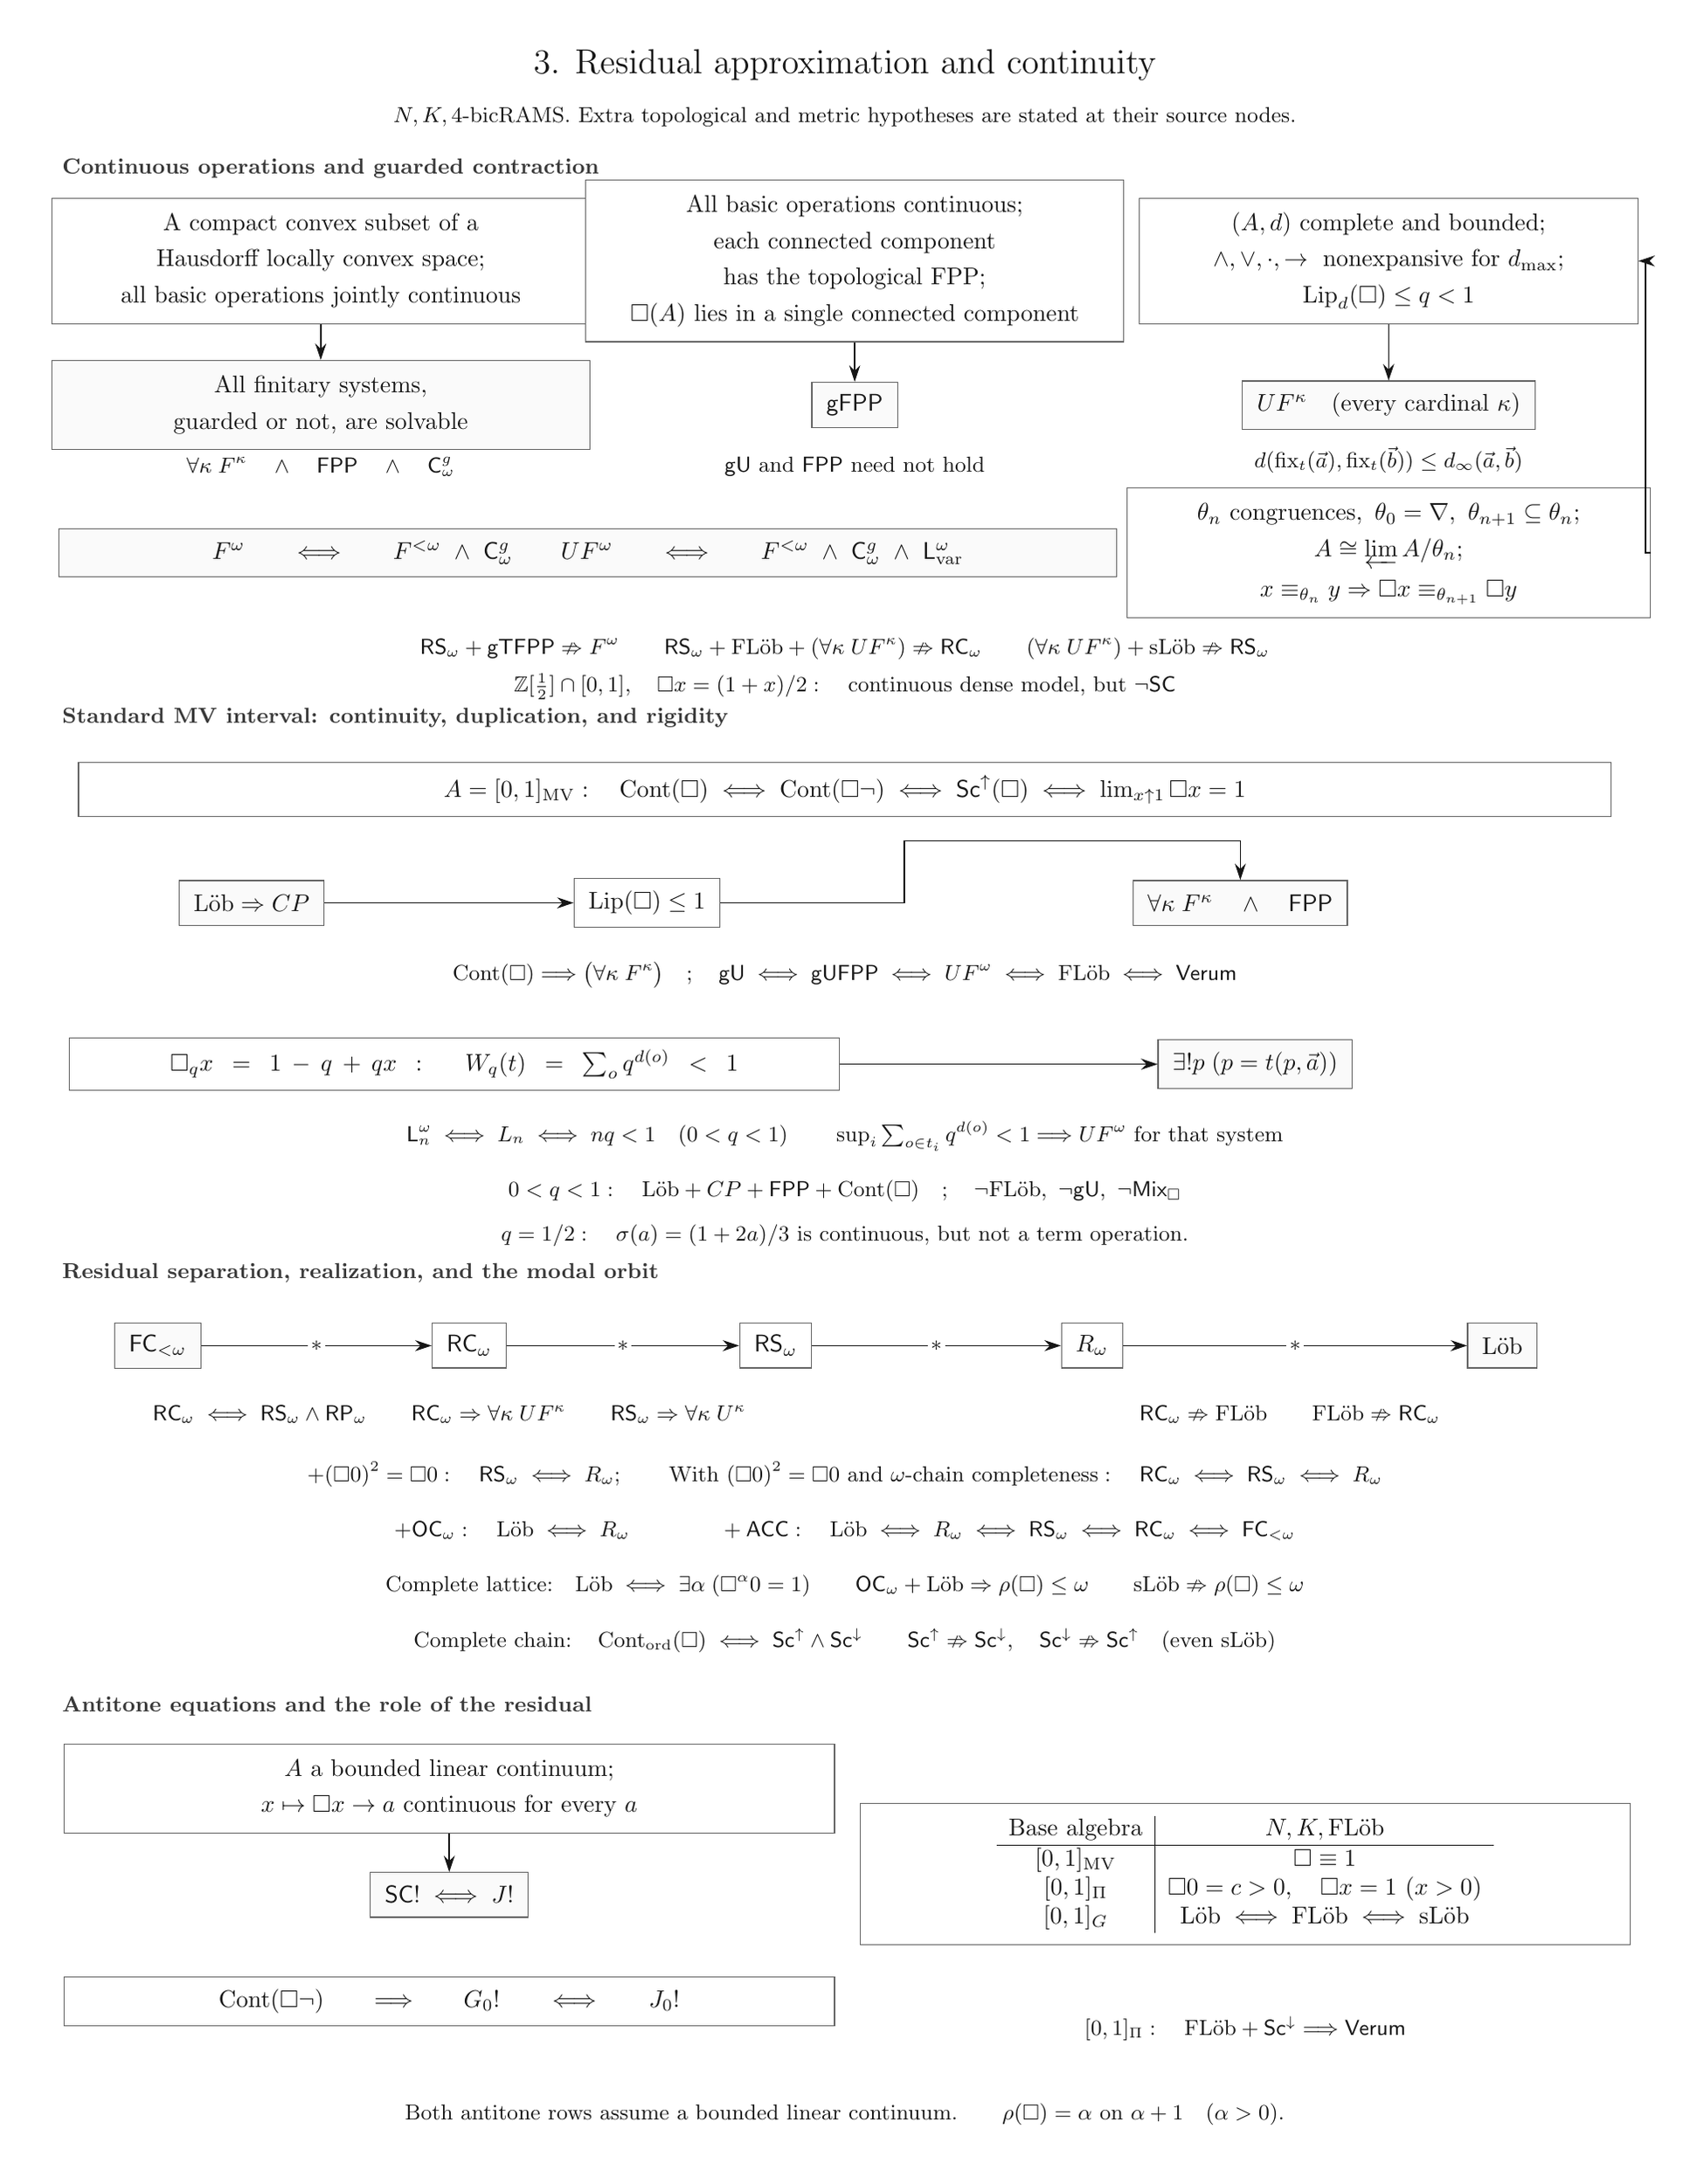
\begin{tikzpicture}[x=.72cm,y=1cm]
\path[use as bounding box] (-.6,-30) rectangle (32.6,1.1);
\Head{3. Residual approximation and continuity}{$N,K,4$-bicRAMS. Extra topological and metric hypotheses are stated at their source nodes.}
\node[title] at (0,-1) {Continuous operations and guarded contraction};
\node[p,text width=7.416cm] (conv) at (5.4,-2.35) {$\begin{gathered}\text{A compact convex subset of a}\\\text{Hausdorff locally convex space;}\\\text{all basic operations jointly continuous}\end{gathered}$};
\node[p,text width=7.416cm] (comp) at (16.2,-2.35) {$\begin{gathered}\text{All basic operations continuous;}\\\text{each connected component}\\\text{has the topological FPP;}\\\Box(A)\text{ lies in a single connected component}\end{gathered}$};
\node[p,text width=6.84cm] (metric) at (27,-2.35) {$\begin{gathered}(A,d)\text{ complete and bounded;}\\\wedge,\vee,\cdot,\to\text{ nonexpansive for }d_{\max};\\\operatorname{Lip}_d(\Box)\le q<1\end{gathered}$};
\node[e,text width=7.416cm] (allconv) at (5.4,-4.45) {$\begin{gathered}\text{All finitary systems,}\\\text{guarded or not, are solvable}\end{gathered}$};
\draw[arr] (conv) -- (allconv);
\node[e] (gcomp) at (16.2,-4.45) {$\gF$};
\draw[arr] (comp) -- (gcomp);
\node[u] (ufmet) at (27,-4.45) {$UF^\kappa\quad(\text{every cardinal }\kappa)$};
\draw[arr] (metric) -- (ufmet);
\node[small] at (5.4,-5.35) {$\forall\kappa\;F^\kappa\quad\wedge\quad\mathsf{FPP}\quad\wedge\quad\mathsf C^g_\omega$};
\node[small] at (16.2,-5.35) {$\gU\text{ and }\mathsf{FPP}\text{ need not hold}$};
\node[small] at (27,-5.25) {$d(\mathrm{fix}_t(\vec a),\mathrm{fix}_t(\vec b))\le d_\infty(\vec a,\vec b)$};
\node[p,text width=7.2cm] (inv) at (27,-6.6) {$\begin{gathered}\theta_n\text{ congruences},\ \theta_0=\nabla,\ \theta_{n+1}\subseteq\theta_n;\\A\cong\varprojlim A/\theta_n;\\x\equiv_{\theta_n}y\Rightarrow\Box x\equiv_{\theta_{n+1}}\Box y\end{gathered}$};
\draw[arr] (inv) -- (32.2,-6.6) -- (32.2,-2.35) -- (metric);
\node[e,text width=14.976cm] (cdec) at (10.8,-6.6) {$F^\omega\iff F^{<\omega}\wedge\mathsf C^g_\omega\qquad UF^\omega\iff F^{<\omega}\wedge\mathsf C^g_\omega\wedge\mathsf L^\omega_{\rm var}$};

\node[small] at (16,-8.0) {$\mathsf{RS}_\omega+\gT\nRightarrow F^\omega\qquad
\mathsf{RS}_\omega+\FL+(\forall\kappa\;UF^\kappa)\nRightarrow\mathsf{RC}_\omega\qquad
(\forall\kappa\;UF^\kappa)+\sL\nRightarrow\mathsf{RS}_\omega$};
\node[small] at (16,-8.55) {$\mathbb Z[\tfrac12]\cap[0,1],\quad\Box x=(1+x)/2:\quad\text{continuous dense model, but }\neg\SC$};

\node[title] at (0,-9) {Standard MV interval: continuity, duplication, and rigidity};
\node[p,minimum width=22.32cm] (mvc) at (16,-10.05) {$A=[0,1]_{\mathrm{MV}}:\quad\operatorname{Cont}(\Box)\iff\operatorname{Cont}(\Box\neg)\iff\mathsf{Sc}^{\uparrow}(\Box)\iff\lim_{x\uparrow1}\Box x=1$};
\node[u] (cp) at (4,-11.7) {$\Lo\Rightarrow CP$};
\node[p] (lip) at (12,-11.7) {$\operatorname{Lip}(\Box)\le1$};
\node[e] (mvf) at (24,-11.7) {$\forall\kappa\;F^\kappa\quad\wedge\quad\mathsf{FPP}$};
\draw[arr] (cp) -- (lip);
\draw[arr] (lip) -- (17.2,-11.7) -- (17.2,-10.8) -- (24,-10.8) -- (mvf);
\node[small] at (16,-12.75) {$\operatorname{Cont}(\Box)\Longrightarrow\bigl(\forall\kappa\;F^\kappa\bigr)\quad;\quad\gU\iff\gUF\iff UF^\omega\iff\FL\iff\Ver$};
\node[p,text width=10.8cm] (weight) at (8.1,-14.05) {$\Box_qx=1-q+qx:\quad W_q(t)=\sum_o q^{d(o)}<1$};
\node[u] (weightuf) at (24.3,-14.05) {$\exists!p\;(p=t(p,\vec a))$};
\draw[arr] (weight) -- (weightuf);
\node[small] at (16,-15.1) {$\mathsf L_n^\omega\iff L_n\iff nq<1\quad(0<q<1)\qquad\sup_i\sum_{o\in t_i}q^{d(o)}<1\Longrightarrow UF^\omega\text{ for that system}$};
\node[small] at (16,-16.55) {$q=1/2:\quad\sigma(a)=(1+2a)/3\text{ is continuous, but not a term operation.}$};
\node[small] at (16,-15.9) {$0<q<1:\quad\Lo+CP+\mathsf{FPP}+\operatorname{Cont}(\Box)\quad;\quad\neg\FL,\ \neg\gU,\ \neg\mathsf{Mix}_{\Box}$};

\node[title] at (0,-17.1) {Residual separation, realization, and the modal orbit};
\node[t] (resfc) at (2.1,-18.15) {$\FC_{<\omega}$};
\node[p] (resrc) at (8.4,-18.15) {$\mathsf{RC}_\omega$};
\node[p] (resrs) at (14.6,-18.15) {$\mathsf{RS}_\omega$};
\node[p] (resr) at (21,-18.15) {$R_\omega$};
\node[u] (resl) at (29.3,-18.15) {$\Lo$};
\draw[arr] (resfc)--node[lab]{$\ast$}(resrc);
\draw[arr] (resrc)--node[lab]{$\ast$}(resrs);
\draw[arr] (resrs)--node[lab]{$\ast$}(resr);
\draw[arr] (resr)--node[lab]{$\ast$}(resl);
\node[small] at (8,-19.15) {$\mathsf{RC}_\omega\iff\mathsf{RS}_\omega\wedge\mathsf{RP}_\omega\qquad\mathsf{RC}_\omega\Rightarrow\forall\kappa\;UF^\kappa\qquad\mathsf{RS}_\omega\Rightarrow\forall\kappa\;U^\kappa$};
\node[small] at (25,-19.15) {$\mathsf{RC}_\omega\nRightarrow\FL\qquad\FL\nRightarrow\mathsf{RC}_\omega$};
\node[small] at (16,-20.05) {$\begin{gathered}
+(\Box0)^2=\Box0:\quad \mathsf{RS}_\omega\iff R_\omega;\qquad
\text{With }(\Box0)^2=\Box0\text{ and }\omega\text{-chain completeness}:\quad \mathsf{RC}_\omega\iff\mathsf{RS}_\omega\iff R_\omega
\end{gathered}$};
\node[small] at (16,-20.85) {$+\mathsf{OC}_\omega:\quad\Lo\iff R_\omega\qquad\qquad
+\mathsf{ACC}:\quad\Lo\iff R_\omega\iff\mathsf{RS}_\omega\iff\mathsf{RC}_\omega\iff\FC_{<\omega}$};
\node[small] at (16,-21.65) {$\text{Complete lattice:}\quad\Lo\iff\exists\alpha\;(\Box^\alpha0=1)\qquad
\mathsf{OC}_\omega+\Lo\Rightarrow\rho(\Box)\le\omega\qquad\sL\nRightarrow\rho(\Box)\le\omega$};
\node[small] at (16,-22.45) {$\text{Complete chain:}\quad
\operatorname{Cont}_{\rm ord}(\Box)\iff\mathsf{Sc}^{\uparrow}\wedge\mathsf{Sc}^{\downarrow}\qquad
\mathsf{Sc}^{\uparrow}\nRightarrow\mathsf{Sc}^{\downarrow},\quad\mathsf{Sc}^{\downarrow}\nRightarrow\mathsf{Sc}^{\uparrow}\quad(\text{even }\sL)$};
\node[title] at (0,-23.4) {Antitone equations and the role of the residual};
\node[p,text width=10.8cm] (anti) at (8,-24.6) {$\begin{gathered}A\text{ a bounded linear continuum;}\\x\mapsto\Box x\to a\text{ continuous for every }a\end{gathered}$};
\node[u] (scanti) at (8,-26.15) {$\SC!\iff J!$};
\draw[arr] (anti) -- (scanti);
\node[p,text width=10.8cm] (janti) at (8,-27.7) {$\operatorname{Cont}(\Box\neg)\quad\Longrightarrow\quad G_0!\iff J_0!$};
\node[p,text width=10.8cm] (bases) at (24.1,-25.85) {$\begin{array}{c|c}\text{Base algebra}&N,K,\FL\\\hline[0,1]_{\mathrm{MV}}&\Box\equiv1\\{}[0,1]_{\Pi}&\Box0=c>0,\quad\Box x=1\ (x>0)\\{}[0,1]_{G}&\Lo\iff\FL\iff\sL\end{array}$};
\node[small] at (24.1,-28.1) {$[0,1]_{\Pi}:\quad\FL+\mathsf{Sc}^{\downarrow}\Longrightarrow\Ver$};
\node[small] at (16,-29.35) {$\text{Both antitone rows assume a bounded linear continuum.}\qquad\rho(\Box)=\alpha\text{ on }\alpha+1\quad(\alpha>0).$};
\end{tikzpicture}

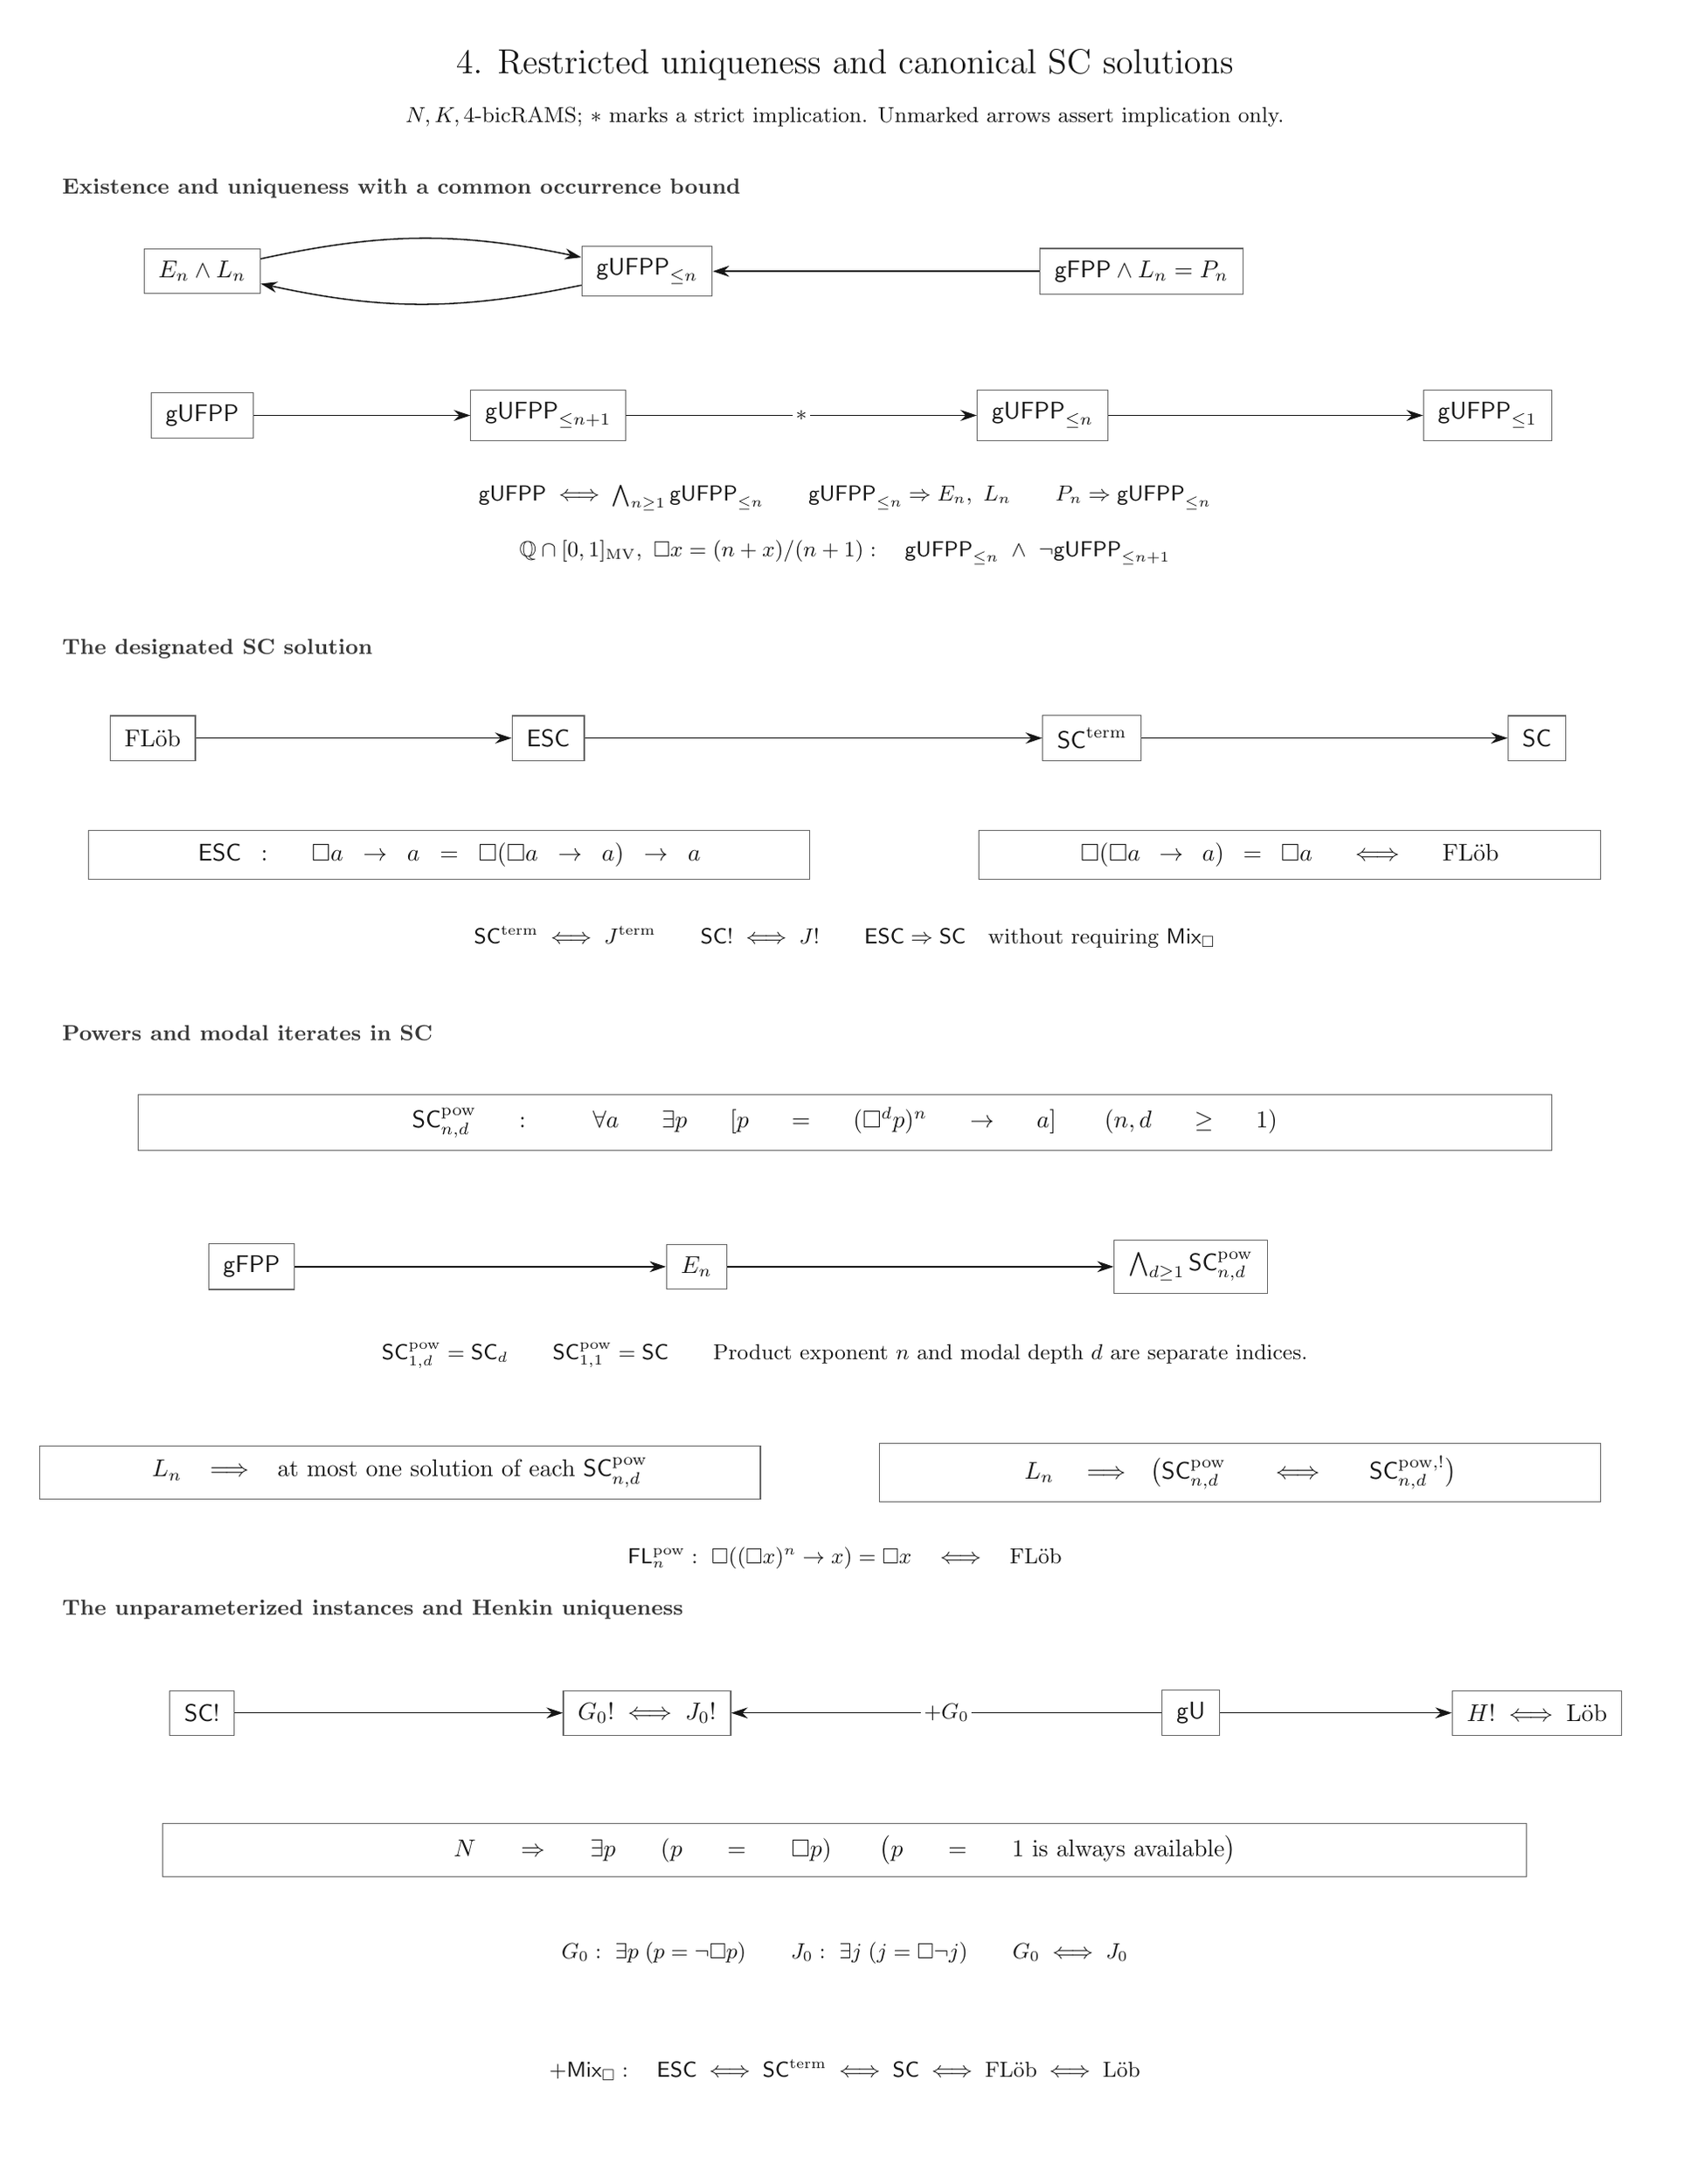
\begin{tikzpicture}[x=.72cm,y=1cm]
\path[use as bounding box] (-.6,-30) rectangle (32.6,1.1);
\Head{4. Restricted uniqueness and canonical SC solutions}{$N,K,4$-bicRAMS; $\ast$ marks a strict implication. Unmarked arrows assert implication only.}
\node[title] at (0,-1.3) {Existence and uniqueness with a common occurrence bound};
\node[p] (r0) at (3,-2.5) {$E_n\wedge L_n$};
\node[p] (r1) at (12,-2.5) {$\mathsf{gUFPP}_{\le n}$};
\node[p] (r2) at (22,-2.5) {$\mathsf{gFPP}\wedge L_n=P_n$};
\draw[arr] (r0) to[bend left=12] (r1);
\draw[arr] (r1) to[bend left=12] (r0);
\draw[arr] (r2) -- (r1);
\node[p] (a) at (3,-4.6) {$\gUF$};
\node[p] (b) at (10,-4.6) {$\mathsf{gUFPP}_{\le n+1}$};
\node[p] (c) at (20,-4.6) {$\mathsf{gUFPP}_{\le n}$};
\node[p] (d) at (29,-4.6) {$\mathsf{gUFPP}_{\le1}$};
\draw[arr] (a) -- (b);
\draw[arr] (b) --node[lab]{$\ast$} (c);
\draw[arr] (c) -- (d);
\node[small] at (16,-5.8) {$\gUF\iff\bigwedge_{n\ge1}\mathsf{gUFPP}_{\le n}\qquad\mathsf{gUFPP}_{\le n}\Rightarrow E_n,\ L_n\qquad P_n\Rightarrow\mathsf{gUFPP}_{\le n}$};
\node[small] at (16,-6.6) {$\mathbb Q\cap[0,1]_{\rm MV},\ \Box x=(n+x)/(n+1):\quad\mathsf{gUFPP}_{\le n}\ \wedge\ \neg\mathsf{gUFPP}_{\le n+1}$};
\node[title] at (0,-8) {The designated SC solution};
\node[p] (f) at (2,-9.3) {$\FL$};
\node[p] (esc) at (10,-9.3) {$\mathsf{ESC}$};
\node[p] (sct) at (21,-9.3) {$\SC^{\rm term}$};
\node[p] (sc) at (30,-9.3) {$\SC$};
\draw[arr] (f) -- (esc);
\draw[arr] (esc) -- (sct);
\draw[arr] (sct) -- (sc);
\node[p,text width=10.08cm] (escid) at (8,-11) {$\mathsf{ESC}:\quad\Box a\to a=\Box(\Box a\to a)\to a$};
\node[p,text width=8.64cm] (jer) at (25,-11) {$\Box(\Box a\to a)=\Box a\quad\Longleftrightarrow\quad\FL$};
\node[small] at (16,-12.2) {$\SC^{\rm term}\iff J^{\rm term}\qquad\SC!\iff J!\qquad\mathsf{ESC}\Rightarrow\SC\quad\text{without requiring }\mathsf{Mix}_{\Box}$};
\node[title] at (0,-13.6) {Powers and modal iterates in SC};
\node[p,text width=20.16cm] (pow) at (16,-14.9) {$\mathsf{SC}^{\rm pow}_{n,d}:\quad\forall a\;\exists p\;[p=(\Box^dp)^n\to a]\qquad(n,d\ge1)$};
\node[p] (gfp) at (4,-17) {$\gF$};
\node[p] (en) at (13,-17) {$E_n$};
\node[p] (pn) at (23,-17) {$\bigwedge_{d\ge1}\mathsf{SC}^{\rm pow}_{n,d}$};
\draw[arr] (gfp) -- (en);
\draw[arr] (en) -- (pn);
\node[small] at (16,-18.3) {$\mathsf{SC}^{\rm pow}_{1,d}=\SC_d\qquad\mathsf{SC}^{\rm pow}_{1,1}=\SC\qquad\text{Product exponent }n\text{ and modal depth }d\text{ are separate indices.}$};
\node[p,text width=10.08cm] (lu) at (7,-20) {$L_n\ \Longrightarrow\ \text{at most one solution of each }\mathsf{SC}^{\rm pow}_{n,d}$};
\node[p,text width=10.08cm] (lue) at (24,-20) {$L_n\ \Longrightarrow\bigl(\mathsf{SC}^{\rm pow}_{n,d}\iff\mathsf{SC}^{\rm pow,!}_{n,d}\bigr)$};
\node[small] at (16,-21.25) {$\mathsf{FL}^{\rm pow}_n:\ \Box((\Box x)^n\to x)=\Box x\quad\Longleftrightarrow\quad\FL$};
\node[title] at (0,-22) {The unparameterized instances and Henkin uniqueness};
\node[p] (st) at (3,-23.5) {$\SC!$};
\node[p] (gt) at (12,-23.5) {$G_0!\iff J_0!$};
\node[p] (gu) at (23,-23.5) {$\gU$};
\node[p] (h) at (30,-23.5) {$H!\iff\Lo$};
\draw[arr] (st) -- (gt);
\draw[arr] (gu) --node[lab]{$+G_0$} (gt);
\draw[arr] (gu) -- (h);
\node[p,text width=19.44cm] (hbase) at (16,-25.5) {$N\Rightarrow\exists p\;(p=\Box p)\qquad\bigl(p=1\text{ is always available}\bigr)$};
\node[small] at (16,-27) {$G_0:\ \exists p\;(p=\neg\Box p)\qquad J_0:\ \exists j\;(j=\Box\neg j)\qquad G_0\iff J_0$};
\node[small] at (16,-28.7) {$+\mathsf{Mix}_{\Box}:\quad\mathsf{ESC}\iff\SC^{\rm term}\iff\SC\iff\FL\iff\Lo$};
\end{tikzpicture}
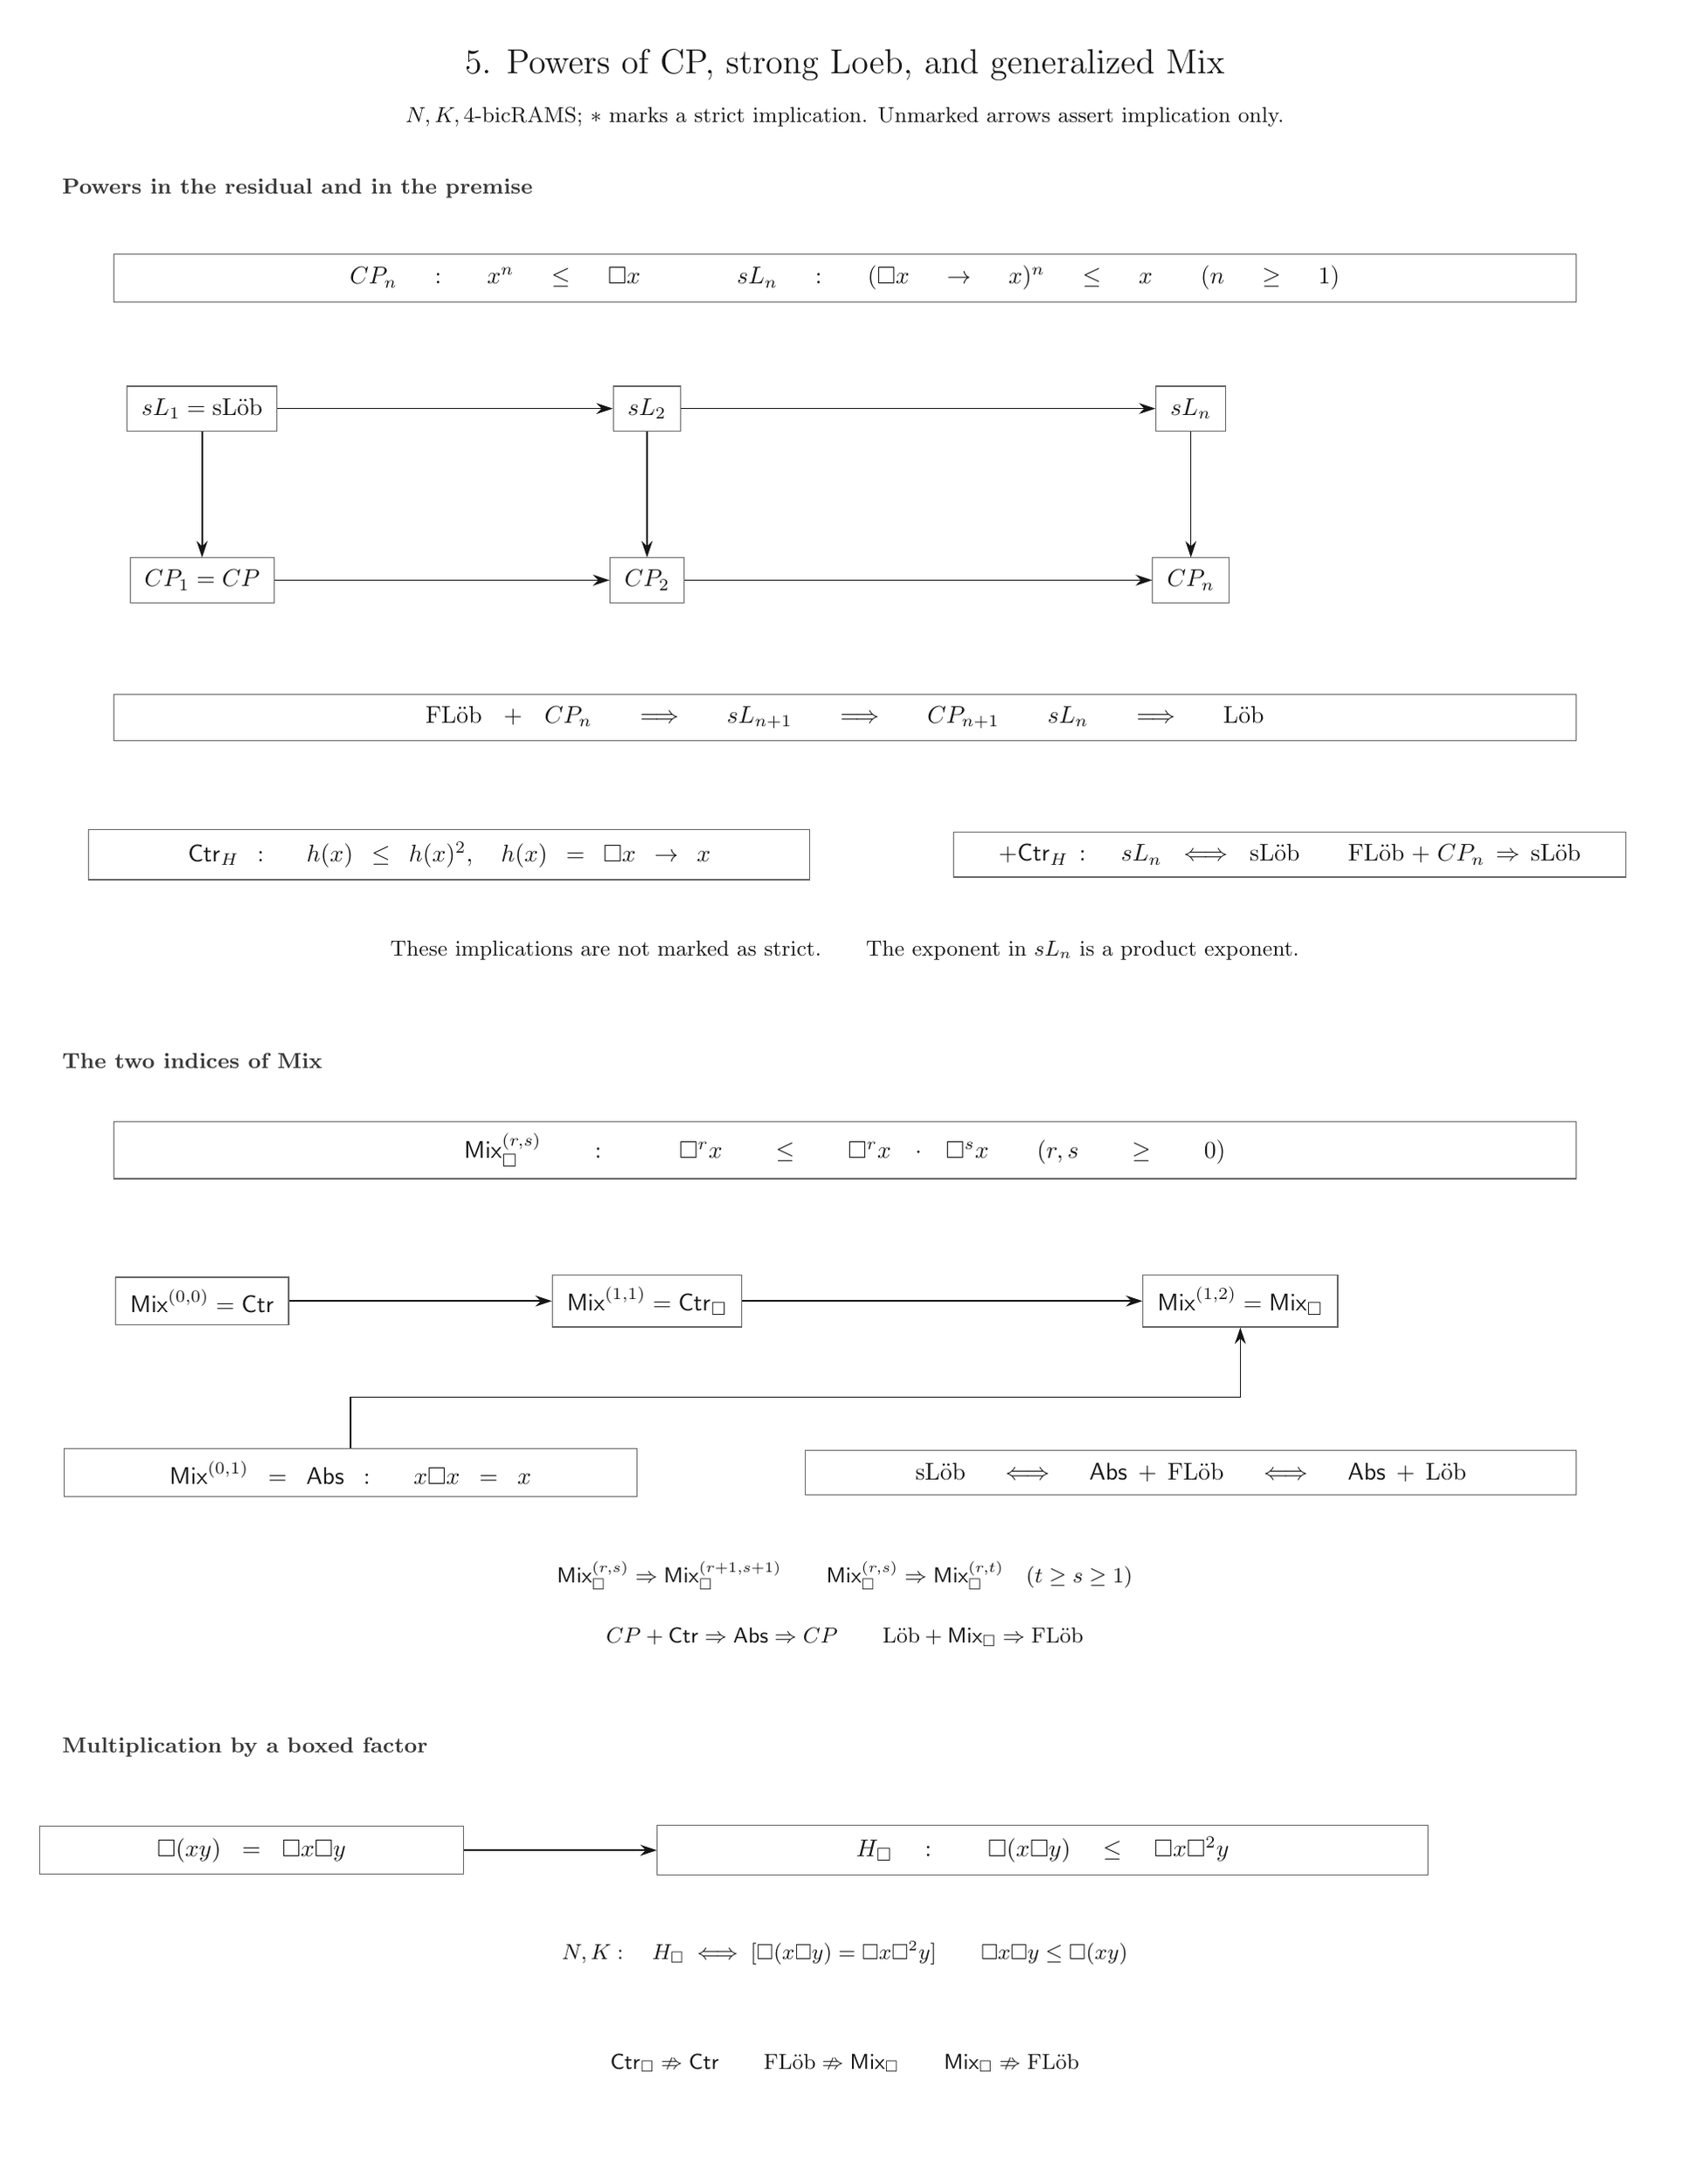
\begin{tikzpicture}[x=.72cm,y=1cm]
\path[use as bounding box] (-.6,-30) rectangle (32.6,1.1);
\Head{5. Powers of CP, strong Loeb, and generalized Mix}{$N,K,4$-bicRAMS; $\ast$ marks a strict implication. Unmarked arrows assert implication only.}
\node[title] at (0,-1.3) {Powers in the residual and in the premise};
\node[p,text width=20.88cm] (defs) at (16,-2.6) {$CP_n:\ x^n\le\Box x\qquad\qquad sL_n:\ (\Box x\to x)^n\le x\qquad(n\ge1)$};
\node[p] (s1) at (3,-4.5) {$sL_1=\sL$};
\node[p] (s2) at (12,-4.5) {$sL_2$};
\node[p] (sn) at (23,-4.5) {$sL_n$};
\node[p] (c1) at (3,-7) {$CP_1=CP$};
\node[p] (c2) at (12,-7) {$CP_2$};
\node[p] (cn) at (23,-7) {$CP_n$};
\draw[arr] (s1) -- (s2);
\draw[arr] (s2) -- (sn);
\draw[arr] (c1) -- (c2);
\draw[arr] (c2) -- (cn);
\draw[arr] (s1) -- (c1);
\draw[arr] (s2) -- (c2);
\draw[arr] (sn) -- (cn);
\node[p,text width=20.88cm] (inter) at (16,-9) {$\FL+CP_n\Longrightarrow sL_{n+1}\Longrightarrow CP_{n+1}\qquad sL_n\Longrightarrow\Lo$};
\node[p,text width=10.08cm] (ch) at (8,-11) {$\mathsf{Ctr}_H:\quad h(x)\le h(x)^2,\quad h(x)=\Box x\to x$};
\node[p,text width=9.36cm] (chc) at (25,-11) {$+\mathsf{Ctr}_H:\quad sL_n\iff\sL\qquad\FL+CP_n\Rightarrow\sL$};
\node[small] at (16,-12.4) {$\text{These implications are not marked as strict.}\qquad \text{The exponent in }sL_n\text{ is a product exponent.}$};
\node[title] at (0,-14) {The two indices of Mix};
\node[p,text width=20.88cm] (mixdef) at (16,-15.3) {$\mathsf{Mix}^{(r,s)}_{\Box}:\quad\Box^rx\le\Box^rx\cdot\Box^sx\qquad(r,s\ge0)$};
\node[p] (ctr) at (3,-17.5) {$\mathsf{Mix}^{(0,0)}=\mathsf{Ctr}$};
\node[p] (ctrb) at (12,-17.5) {$\mathsf{Mix}^{(1,1)}=\mathsf{Ctr}_{\Box}$};
\node[p] (mix) at (24,-17.5) {$\mathsf{Mix}^{(1,2)}=\mathsf{Mix}_{\Box}$};
\draw[arr] (ctr) -- (ctrb);
\draw[arr] (ctrb) -- (mix);
\node[p,text width=7.92cm] (abs) at (6,-20) {$\mathsf{Mix}^{(0,1)}=\Abs:\quad x\Box x=x$};
\node[p,text width=10.8cm] (sl) at (23,-20) {$\sL\iff\Abs+\FL\iff\Abs+\Lo$};
\draw[arr] (abs) -- (6,-18.9) -- (24,-18.9) -- (mix);
\node[small] at (16,-21.5) {$\mathsf{Mix}^{(r,s)}_{\Box}\Rightarrow\mathsf{Mix}^{(r+1,s+1)}_{\Box}\qquad\mathsf{Mix}^{(r,s)}_{\Box}\Rightarrow\mathsf{Mix}^{(r,t)}_{\Box}\quad(t\ge s\ge1)$};
\node[small] at (16,-22.4) {$CP+\mathsf{Ctr}\Rightarrow\Abs\Rightarrow CP\qquad\Lo+\mathsf{Mix}_{\Box}\Rightarrow\FL$};
\node[title] at (0,-24) {Multiplication by a boxed factor};
\node[p,text width=5.76cm] (mult) at (4,-25.5) {$\Box(xy)=\Box x\Box y$};
\node[p,text width=10.8cm] (hbox) at (20,-25.5) {$H_{\Box}:\quad\Box(x\Box y)\le\Box x\Box^2y$};
\draw[arr] (mult) -- (hbox);
\node[small] at (16,-27) {$N,K:\quad H_{\Box}\iff[\Box(x\Box y)=\Box x\Box^2y]\qquad\Box x\Box y\le\Box(xy)$};
\node[small] at (16,-28.6) {$\mathsf{Ctr}_{\Box}\nRightarrow\mathsf{Ctr}\qquad\FL\nRightarrow\mathsf{Mix}_{\Box}\qquad\mathsf{Mix}_{\Box}\nRightarrow\FL$};
\end{tikzpicture}
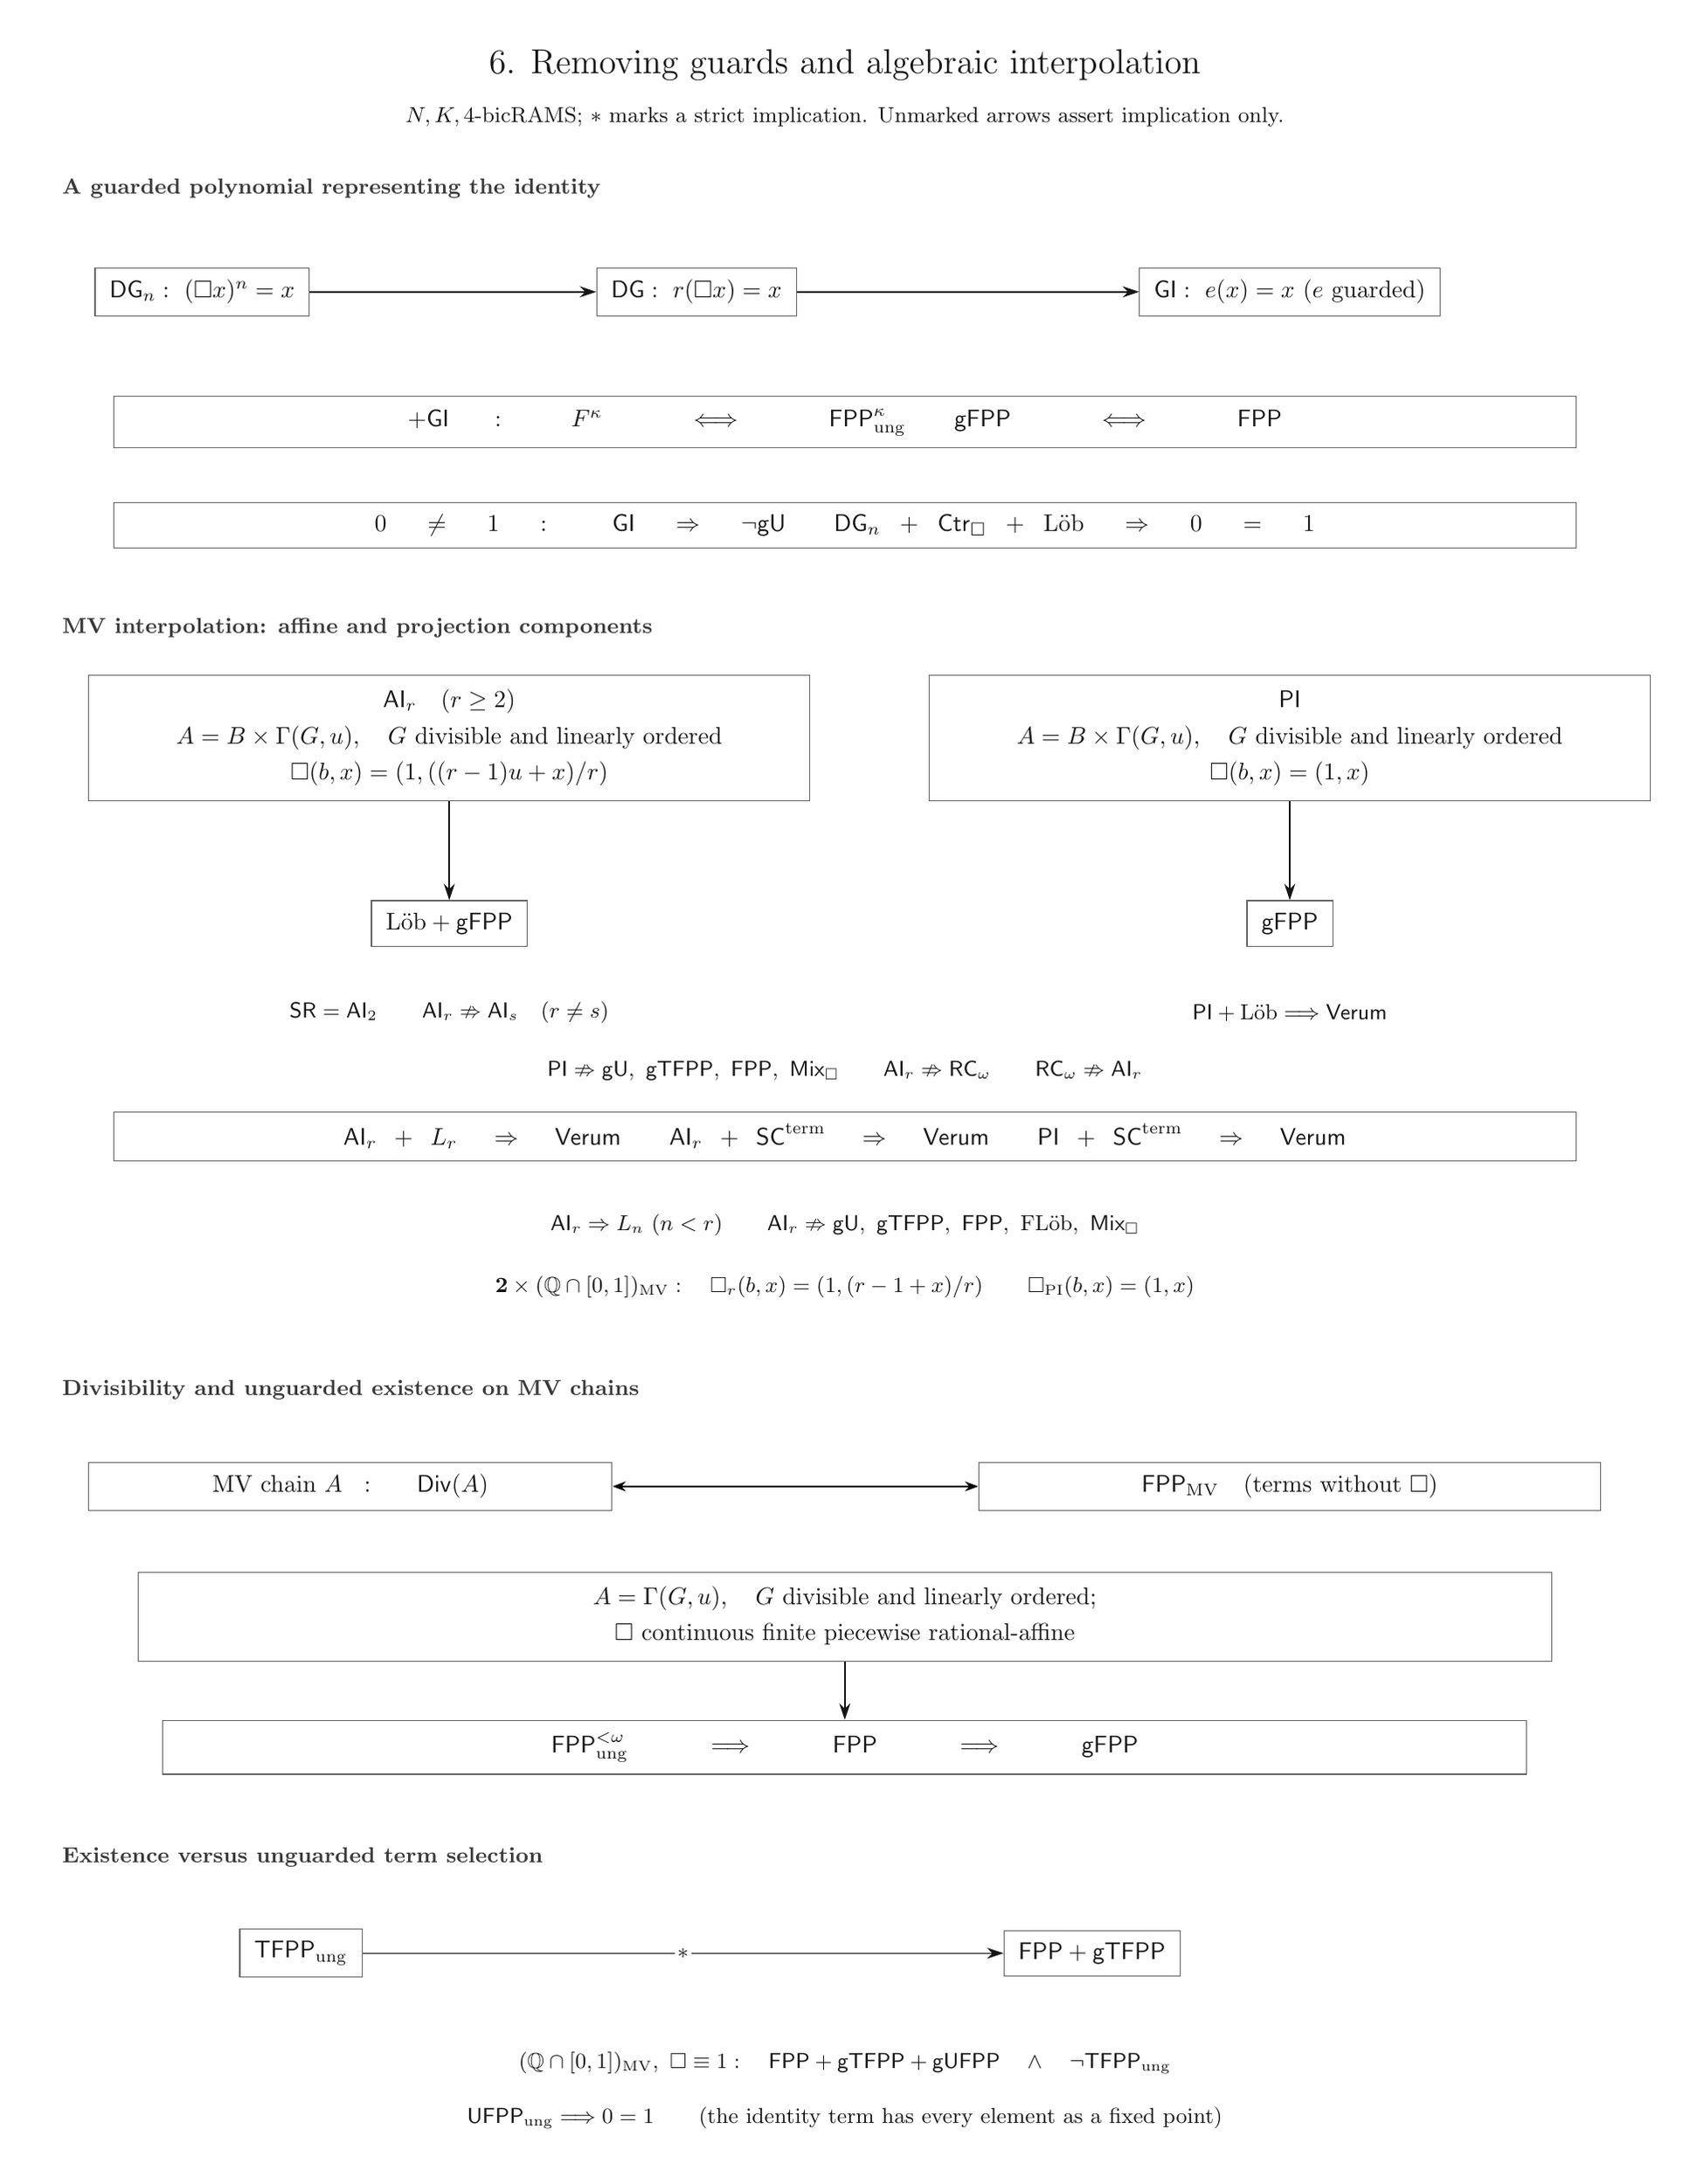
\begin{tikzpicture}[x=.72cm,y=1cm]
\path[use as bounding box] (-.6,-30) rectangle (32.6,1.1);
\Head{6. Removing guards and algebraic interpolation}{$N,K,4$-bicRAMS; $\ast$ marks a strict implication. Unmarked arrows assert implication only.}
\node[title] at (0,-1.3) {A guarded polynomial representing the identity};
\node[p] (dgN) at (3,-2.8) {$\mathsf{DG}_n:\ (\Box x)^n=x$};
\node[p] (dg) at (13,-2.8) {$\mathsf{DG}:\ r(\Box x)=x$};
\node[p] (gi) at (25,-2.8) {$\mathsf{GI}:\ e(x)=x\ (e\text{ guarded})$};
\draw[arr] (dgN) -- (dg);
\draw[arr] (dg) -- (gi);
\node[p,text width=20.88cm] (deguard) at (16,-4.7) {$+\mathsf{GI}:\quad F^\kappa\iff\mathsf{FPP}^{\kappa}_{\rm ung}\qquad\gF\iff\mathsf{FPP}$};
\node[p,text width=20.88cm] (nugi) at (16,-6.2) {$0\ne1:\quad\mathsf{GI}\Rightarrow\neg\gU\qquad\mathsf{DG}_n+\mathsf{Ctr}_{\Box}+\Lo\Rightarrow0=1$};
\node[title] at (0,-7.7) {MV interpolation: affine and projection components};
\node[p,text width=10.08cm] (ai) at (8,-9.3) {$\begin{gathered}\mathsf{AI}_r\quad(r\ge2)\\A=B\times\Gamma(G,u),\quad G\text{ divisible and linearly ordered}\\\Box(b,x)=(1,((r-1)u+x)/r)\end{gathered}$};
\node[p,text width=10.08cm] (pi) at (25,-9.3) {$\begin{gathered}\mathsf{PI}\\A=B\times\Gamma(G,u),\quad G\text{ divisible and linearly ordered}\\\Box(b,x)=(1,x)\end{gathered}$};
\node[p] (aif) at (8,-12) {$\Lo+\gF$};
\node[p] (pif) at (25,-12) {$\gF$};
\draw[arr] (ai) -- (aif);
\draw[arr] (pi) -- (pif);
\node[small] at (8,-13.3) {$\mathsf{SR}=\mathsf{AI}_2\qquad\mathsf{AI}_r\nRightarrow\mathsf{AI}_s\quad(r\ne s)$};
\node[small] at (25,-13.3) {$\mathsf{PI}+\Lo\Longrightarrow\Ver$};
\node[small] at (16,-14.15) {$\mathsf{PI}\nRightarrow\gU,\ \gT,\ \mathsf{FPP},\ \mathsf{Mix}_{\Box}\qquad\mathsf{AI}_r\nRightarrow\mathsf{RC}_\omega\qquad\mathsf{RC}_\omega\nRightarrow\mathsf{AI}_r$};
\node[p,text width=20.88cm] (airef) at (16,-15.1) {$\mathsf{AI}_r+L_r\Rightarrow\Ver\qquad\mathsf{AI}_r+\SC^{\rm term}\Rightarrow\Ver\qquad\mathsf{PI}+\SC^{\rm term}\Rightarrow\Ver$};
\node[small] at (16,-16.4) {$\mathsf{AI}_r\Rightarrow L_n\ (n<r)\qquad\mathsf{AI}_r\nRightarrow\gU,\ \gT,\ \mathsf{FPP},\ \FL,\ \mathsf{Mix}_{\Box}$};
\node[small] at (16,-17.3) {$\mathbf2\times(\mathbb Q\cap[0,1])_{\rm MV}:\quad\Box_r(b,x)=(1,(r-1+x)/r)\qquad\Box_{\rm PI}(b,x)=(1,x)$};
\node[title] at (0,-18.8) {Divisibility and unguarded existence on MV chains};
\node[p,text width=7.2cm] (div) at (6,-20.2) {$\text{MV chain }A:\quad\mathsf{Div}(A)$};
\node[p,text width=8.64cm] (basef) at (25,-20.2) {$\mathsf{FPP}_{\rm MV}\quad\text{(terms without }\Box\text{)}$};
\draw[eq] (div) -- (basef);
\node[p,text width=20.16cm] (aff) at (16,-22.1) {$\begin{gathered}A=\Gamma(G,u),\quad G\text{ divisible and linearly ordered};\\\Box\text{ continuous finite piecewise rational-affine}\end{gathered}$};
\node[p,text width=19.44cm] (afff) at (16,-24) {$\mathsf{FPP}^{<\omega}_{\rm ung}\quad\Longrightarrow\quad\mathsf{FPP}\quad\Longrightarrow\quad\gF$};
\draw[arr] (aff) -- (afff);
\node[title] at (0,-25.6) {Existence versus unguarded term selection};
\node[p] (tung) at (5,-27) {$\mathsf{TFPP}_{\rm ung}$};
\node[p] (tungf) at (21,-27) {$\mathsf{FPP}+\gT$};
\draw[arr] (tung) --node[lab]{$\ast$} (tungf);
\node[small] at (16,-29.4) {$\mathsf{UFPP}_{\rm ung}\Longrightarrow0=1\qquad\text{(the identity term has every element as a fixed point)}$};
\node[small] at (16,-28.6) {$(\mathbb Q\cap[0,1])_{\rm MV},\ \Box\equiv1:\quad\mathsf{FPP}+\gT+\gUF\quad\wedge\quad\neg\mathsf{TFPP}_{\rm ung}$};
\end{tikzpicture}
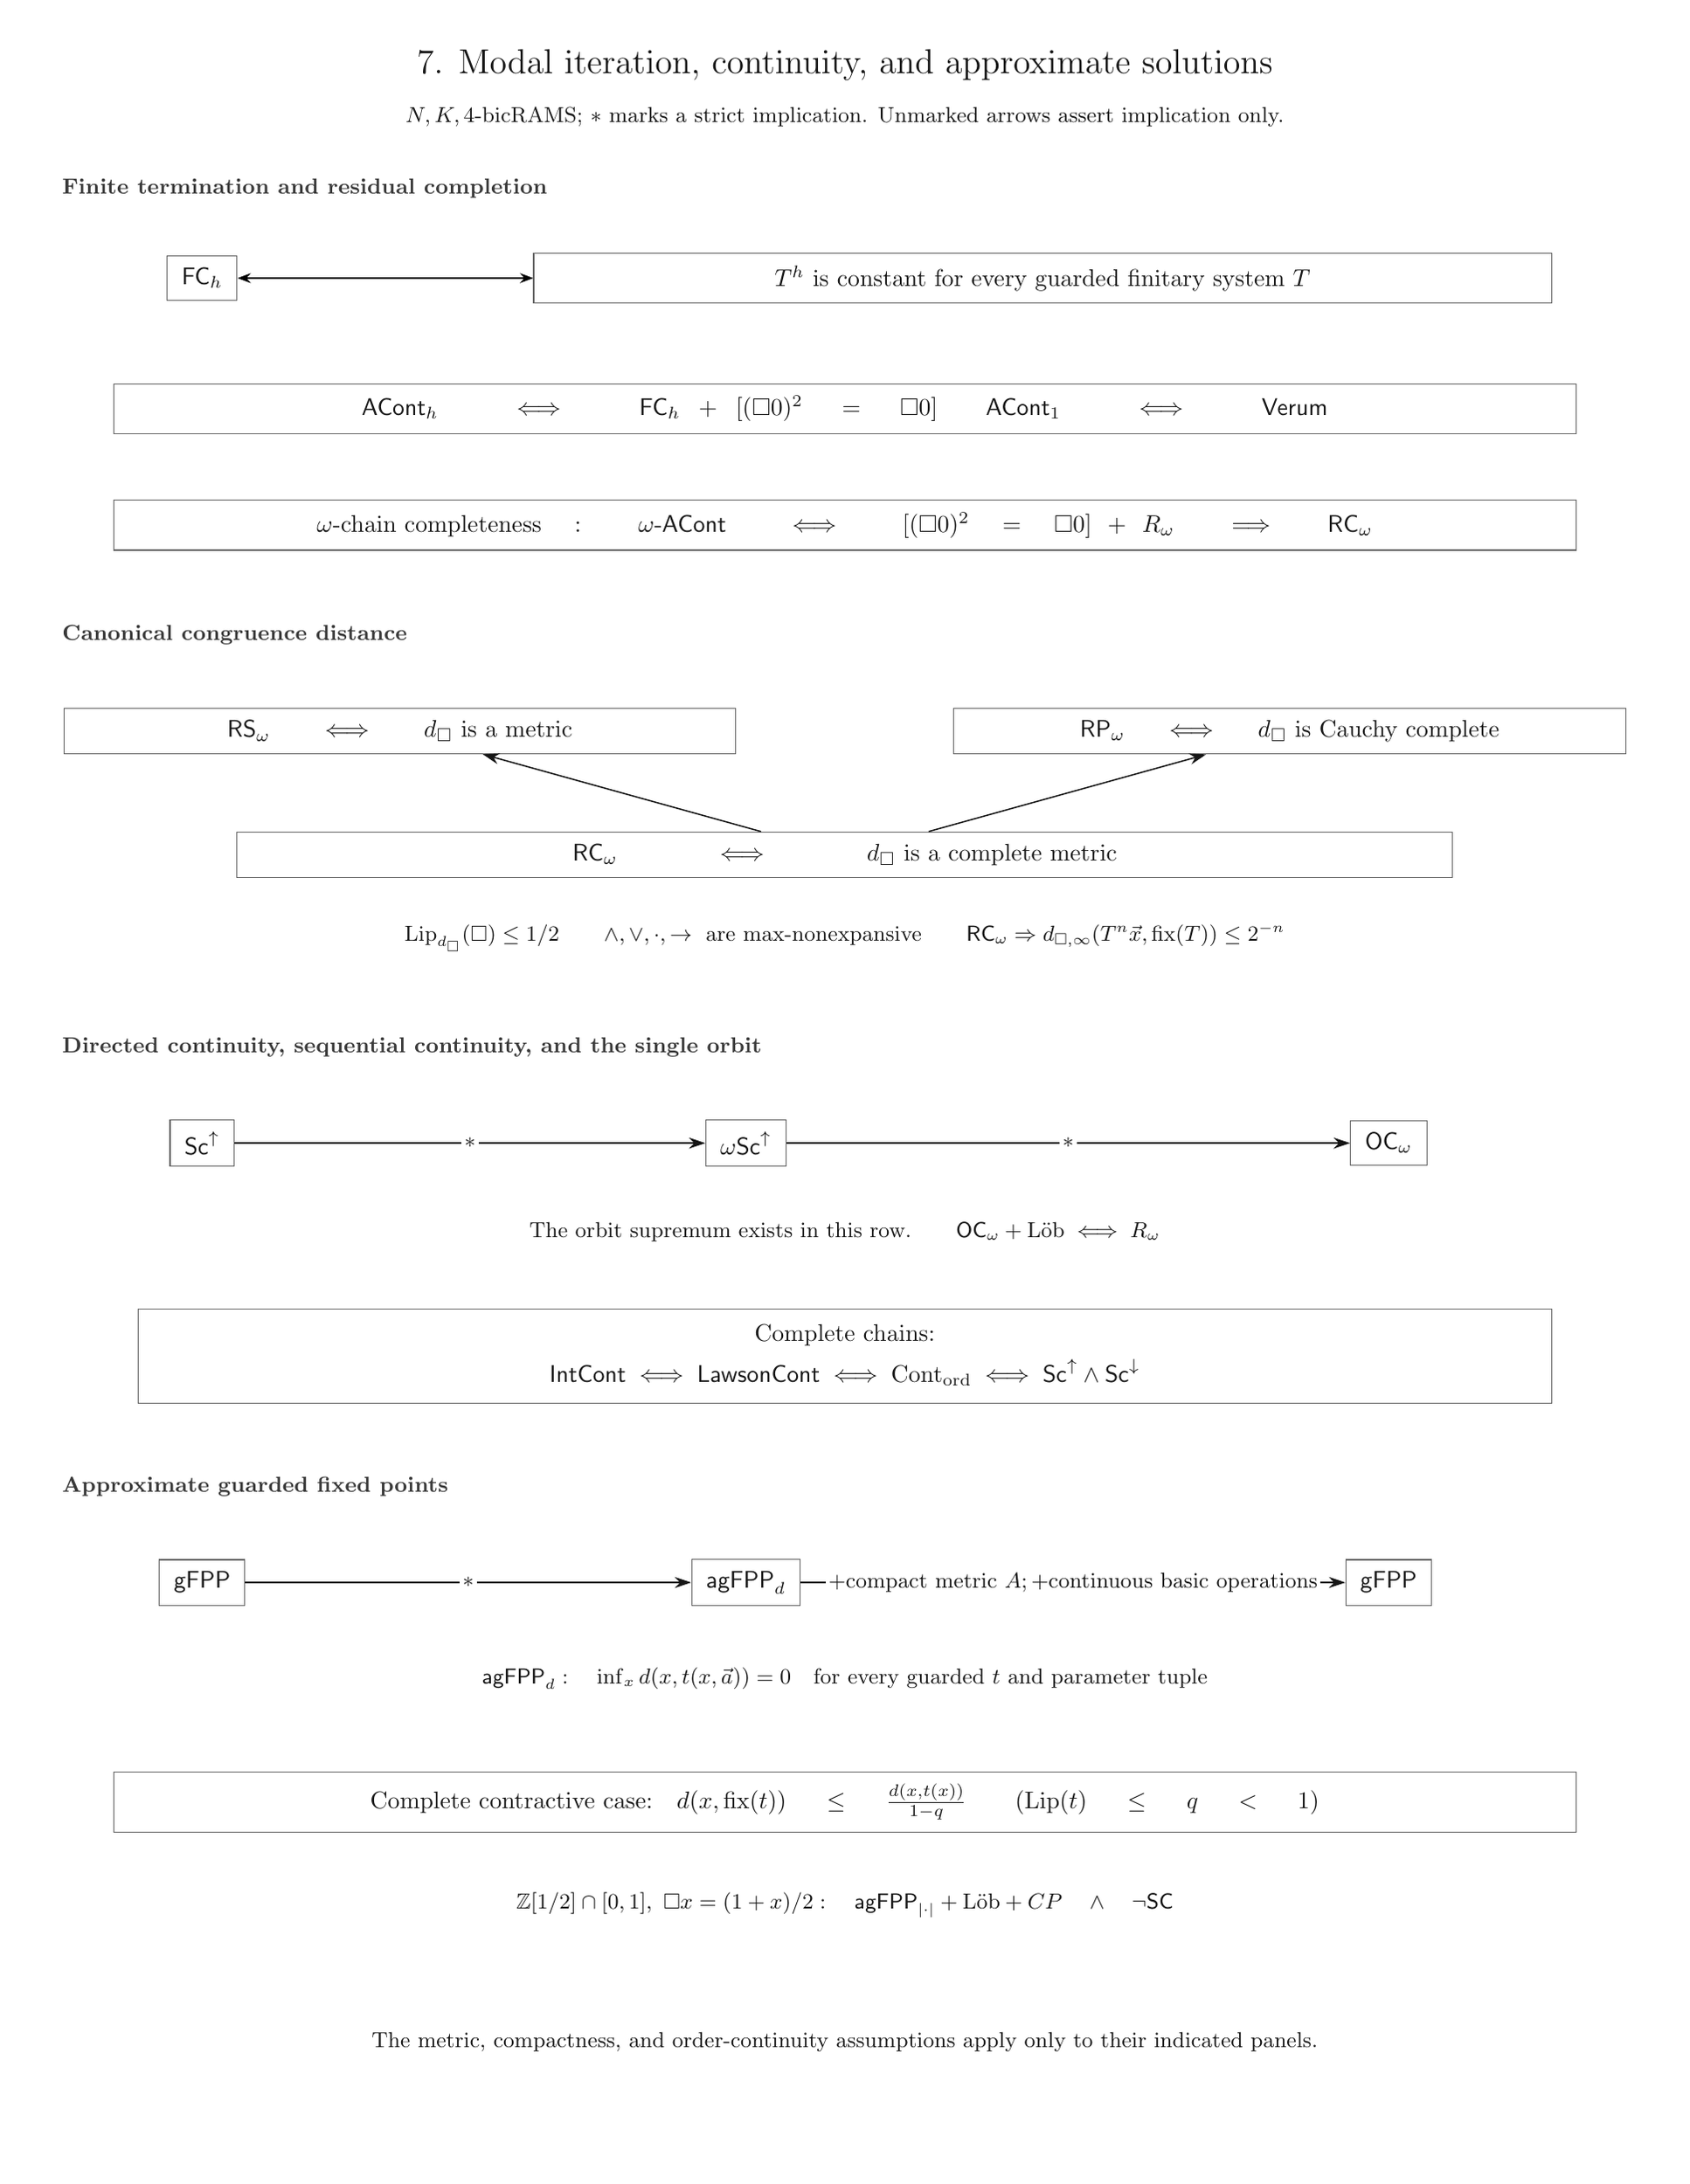
\begin{tikzpicture}[x=.72cm,y=1cm]
\path[use as bounding box] (-.6,-30) rectangle (32.6,1.1);
\Head{7. Modal iteration, continuity, and approximate solutions}{$N,K,4$-bicRAMS; $\ast$ marks a strict implication. Unmarked arrows assert implication only.}
\node[title] at (0,-1.3) {Finite termination and residual completion};
\node[p] (fc) at (3,-2.6) {$\FC_h$};
\node[p,text width=14.4cm] (iter) at (20,-2.6) {$T^h\text{ is constant for every guarded finitary system }T$};
\draw[eq] (fc) -- (iter);
\node[p,text width=20.88cm] (ac) at (16,-4.5) {$\mathsf{ACont}_h\iff\FC_h+[(\Box0)^2=\Box0]\qquad\mathsf{ACont}_1\iff\Ver$};
\node[p,text width=20.88cm] (wac) at (16,-6.2) {$\omega\text{-chain completeness}:\quad\omega\text{-}\mathsf{ACont}\iff[(\Box0)^2=\Box0]+R_\omega\quad\Longrightarrow\quad\mathsf{RC}_\omega$};
\node[title] at (0,-7.8) {Canonical congruence distance};
\node[p,text width=9.36cm] (rsc) at (7,-9.2) {$\mathsf{RS}_\omega\iff d_{\Box}\text{ is a metric}$};
\node[p,text width=9.36cm] (rpc) at (25,-9.2) {$\mathsf{RP}_\omega\iff d_{\Box}\text{ is Cauchy complete}$};
\node[p,text width=17.28cm] (rcc) at (16,-11) {$\mathsf{RC}_\omega\iff d_{\Box}\text{ is a complete metric}$};
\draw[arr] (rcc) -- (rsc);
\draw[arr] (rcc) -- (rpc);
\node[small] at (16,-12.2) {$\operatorname{Lip}_{d_{\Box}}(\Box)\le1/2\qquad\wedge,\vee,\cdot,\to\text{ are max-nonexpansive}\qquad\mathsf{RC}_\omega\Rightarrow d_{\Box,\infty}(T^n\vec x,\mathrm{fix}(T))\le2^{-n}$};
\node[title] at (0,-13.8) {Directed continuity, sequential continuity, and the single orbit};
\node[p] (sc) at (3,-15.2) {$\mathsf{Sc}^{\uparrow}$};
\node[p] (wsc) at (14,-15.2) {$\omega\mathsf{Sc}^{\uparrow}$};
\node[p] (oc) at (27,-15.2) {$\mathsf{OC}_\omega$};
\draw[arr] (sc) --node[lab]{$\ast$} (wsc);
\draw[arr] (wsc) --node[lab]{$\ast$} (oc);
\node[small] at (16,-16.5) {$\text{The orbit supremum exists in this row.}\qquad\mathsf{OC}_\omega+\Lo\iff R_\omega$};
\node[p,text width=20.16cm] (ctop) at (16,-18.3) {$\begin{gathered}\text{Complete chains:}\\\mathsf{IntCont}\iff\mathsf{LawsonCont}\iff\operatorname{Cont}_{\rm ord}\iff\mathsf{Sc}^{\uparrow}\wedge\mathsf{Sc}^{\downarrow}\end{gathered}$};
\node[title] at (0,-20.2) {Approximate guarded fixed points};
\node[p] (ex) at (3,-21.6) {$\gF$};
\node[p] (ap) at (14,-21.6) {$\mathsf{agFPP}_d$};
\node[p] (cl) at (27,-21.6) {$\gF$};
\draw[arr] (ex) --node[lab]{$\ast$} (ap);
\draw[arr] (ap)--node[lab]{$+\text{compact metric }A;+\text{continuous basic operations}$}(cl);
\node[small] at (16,-23) {$\mathsf{agFPP}_d:\quad\inf_x d(x,t(x,\vec a))=0\quad\text{for every guarded }t\text{ and parameter tuple}$};
\node[p,text width=20.88cm] (error) at (16,-24.8) {$\text{Complete contractive case:}\quad d(x,\mathrm{fix}(t))\le\frac{d(x,t(x))}{1-q}\qquad(\operatorname{Lip}(t)\le q<1)$};
\node[small] at (16,-26.3) {$\mathbb Z[1/2]\cap[0,1],\ \Box x=(1+x)/2:\quad\mathsf{agFPP}_{|\cdot|}+\Lo+CP\quad\wedge\quad\neg\SC$};
\node[small] at (16,-28.3) {$\text{The metric, compactness, and order-continuity assumptions apply only to their indicated panels.}$};
\end{tikzpicture}
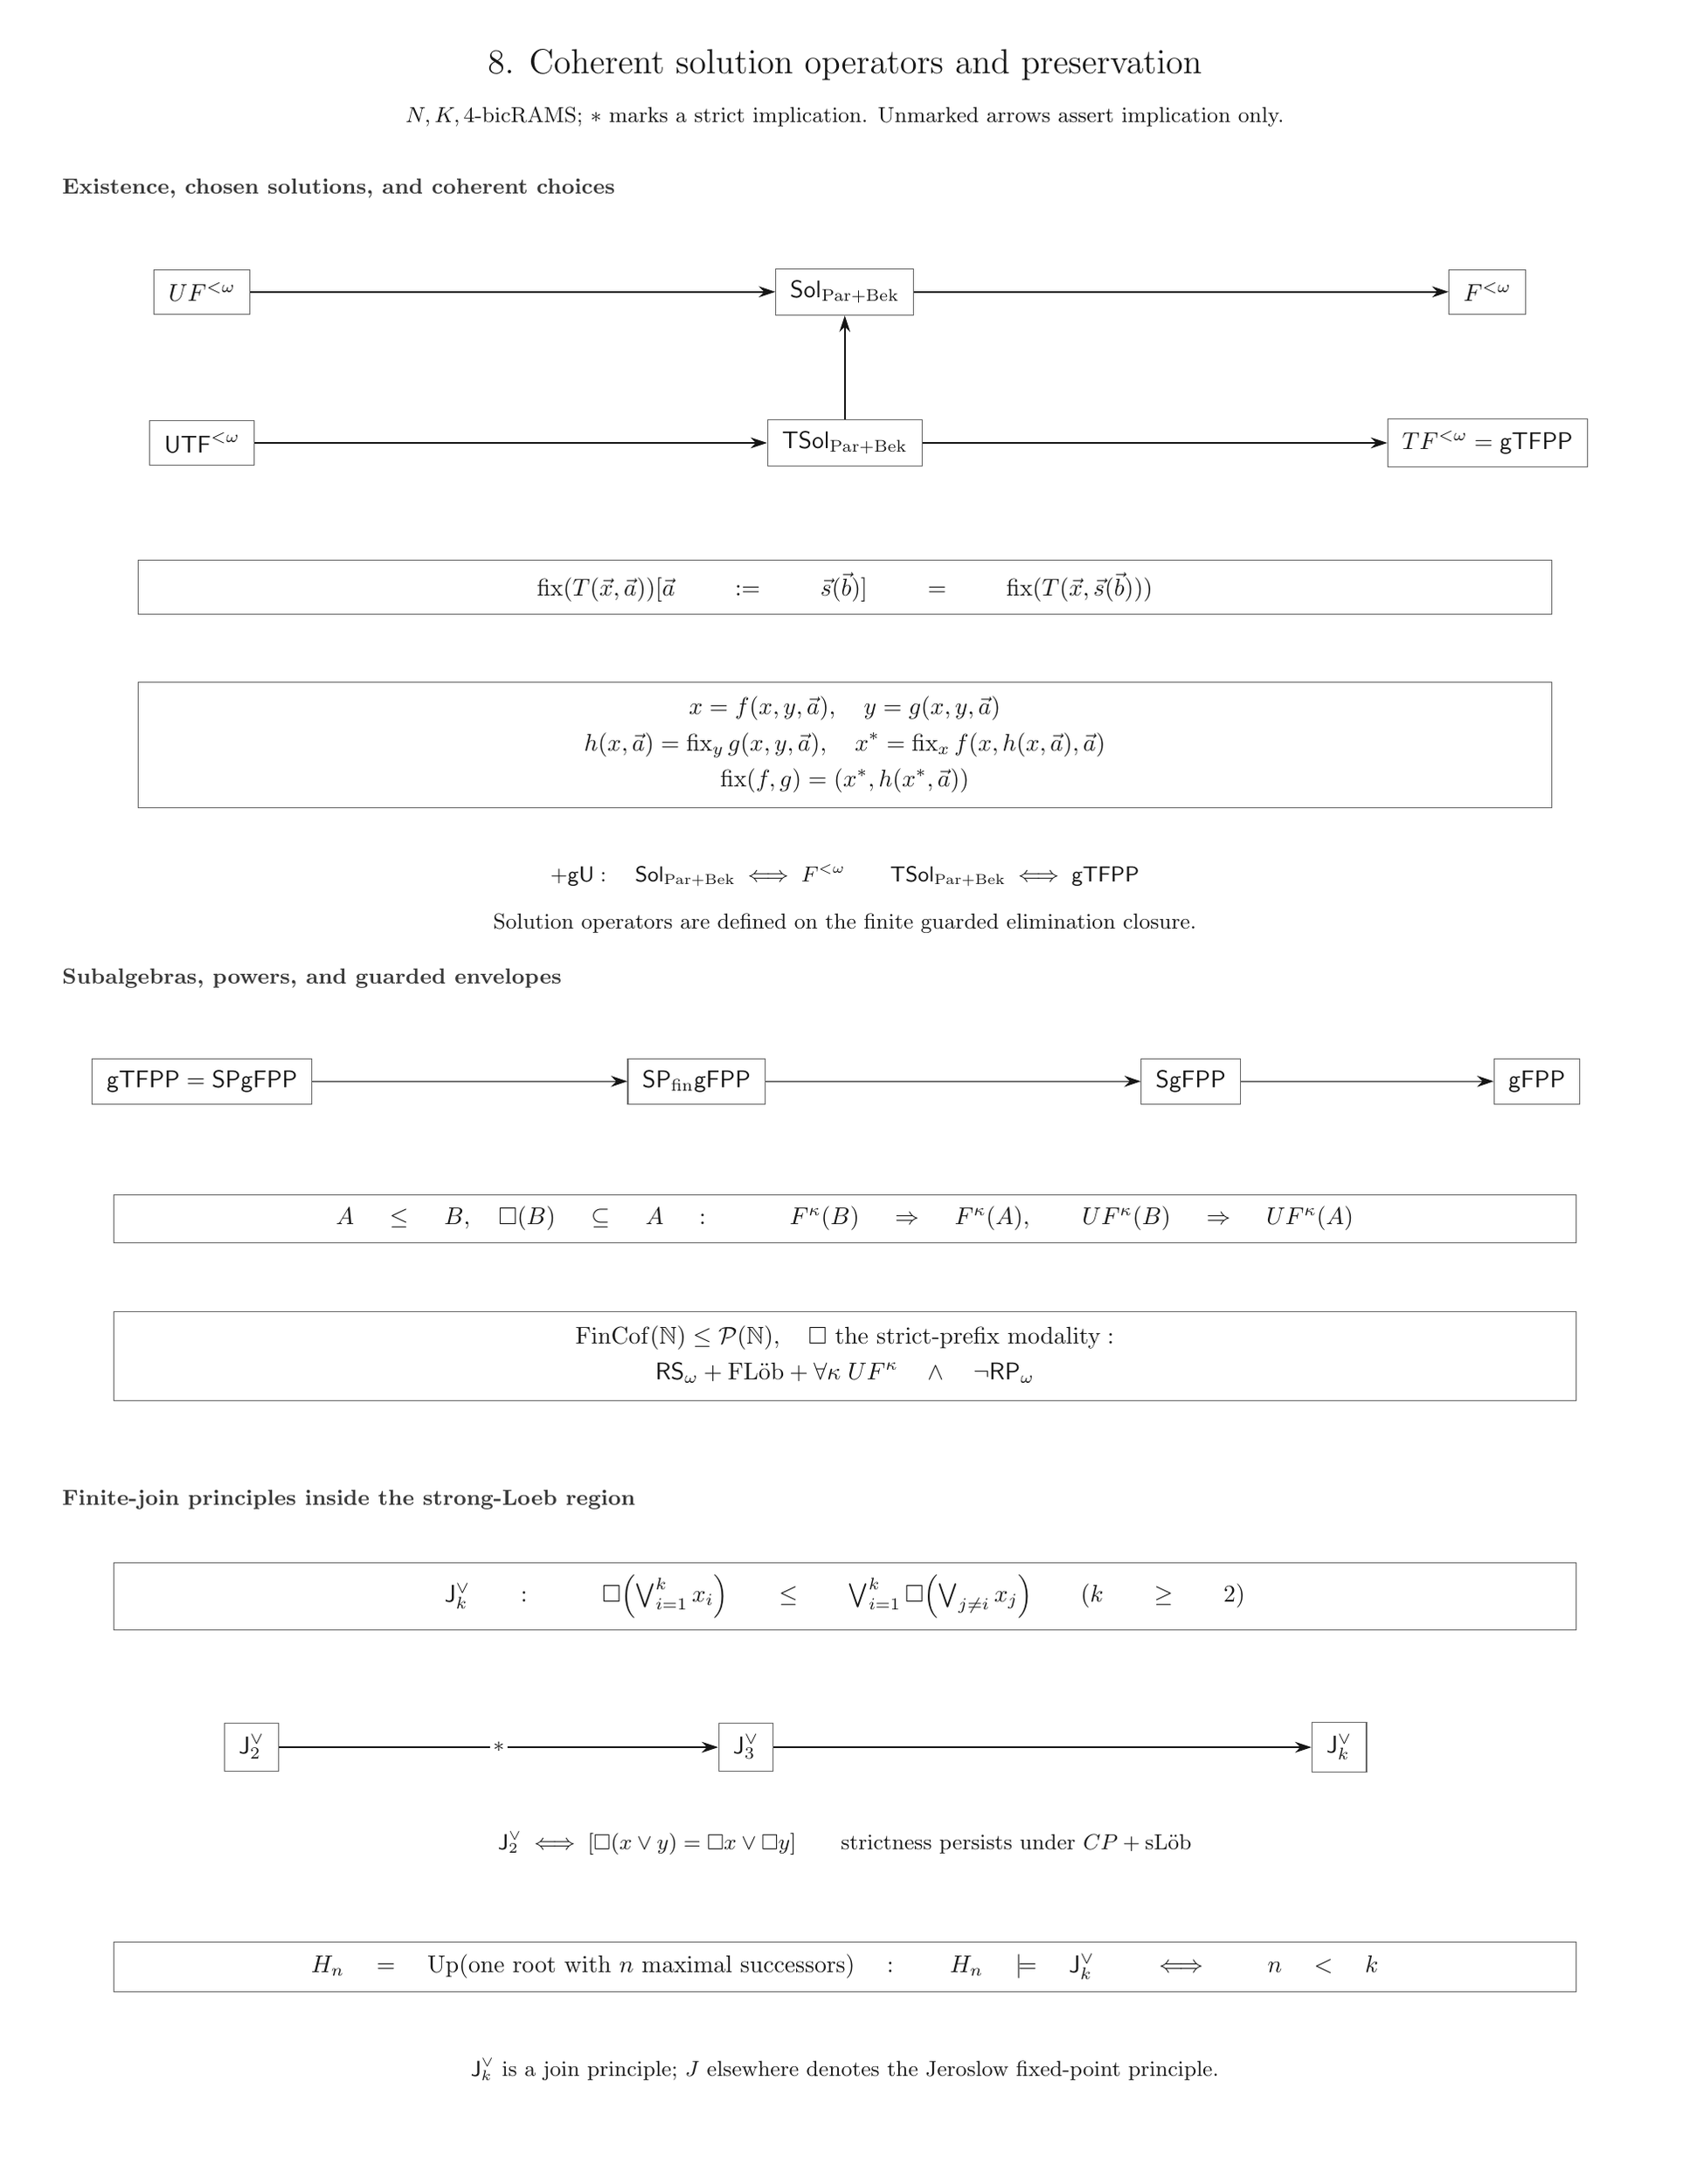
\begin{tikzpicture}[x=.72cm,y=1cm]
\path[use as bounding box] (-.6,-30) rectangle (32.6,1.1);
\Head{8. Coherent solution operators and preservation}{$N,K,4$-bicRAMS; $\ast$ marks a strict implication. Unmarked arrows assert implication only.}
\node[title] at (0,-1.3) {Existence, chosen solutions, and coherent choices};
\node[p] (uf) at (3,-2.8) {$UF^{<\omega}$};
\node[p] (bek) at (16,-2.8) {$\mathsf{Sol}_{\rm Par+Bek}$};
\node[p] (finite) at (29,-2.8) {$F^{<\omega}$};
\draw[arr] (uf) -- (bek);
\draw[arr] (bek) -- (finite);
\node[p] (utf) at (3,-5) {$\UTF^{<\omega}$};
\node[p] (tbek) at (16,-5) {$\mathsf{TSol}_{\rm Par+Bek}$};
\node[p] (tf) at (29,-5) {$TF^{<\omega}=\gT$};
\draw[arr] (utf) -- (tbek);
\draw[arr] (tbek) -- (tf);
\draw[arr] (tbek) -- (bek);
\node[p,text width=20.16cm] (par) at (16,-7.1) {$\mathrm{fix}(T(\vec x,\vec a))[\vec a:=\vec s(\vec b)]=\mathrm{fix}(T(\vec x,\vec s(\vec b)))$};
\node[p,text width=20.16cm] (bk) at (16,-9.4) {$\begin{gathered}x=f(x,y,\vec a),\quad y=g(x,y,\vec a)\\h(x,\vec a)=\mathrm{fix}_y\,g(x,y,\vec a),\quad x^*=\mathrm{fix}_x\,f(x,h(x,\vec a),\vec a)\\\mathrm{fix}(f,g)=(x^*,h(x^*,\vec a))\end{gathered}$};
\node[small] at (16,-11.3) {$+\gU:\quad\mathsf{Sol}_{\rm Par+Bek}\iff F^{<\omega}\qquad\mathsf{TSol}_{\rm Par+Bek}\iff\gT$};
\node[small] at (16,-12) {$\text{Solution operators are defined on the finite guarded elimination closure.}$};
\node[title] at (0,-12.8) {Subalgebras, powers, and guarded envelopes};
\node[p] (sp) at (3,-14.3) {$\gT=\mathsf{SPgFPP}$};
\node[p] (spfin) at (13,-14.3) {$\mathsf{SP}_{\rm fin}\gF$};
\node[p] (sg) at (23,-14.3) {$\mathsf{SgFPP}$};
\node[p] (gf) at (30,-14.3) {$\gF$};
\draw[arr] (sp) -- (spfin);
\draw[arr] (spfin) -- (sg);
\draw[arr] (sg) -- (gf);
\node[p,text width=20.88cm] (env) at (16,-16.3) {$A\le B,\quad\Box(B)\subseteq A:\qquad F^\kappa(B)\Rightarrow F^\kappa(A),\qquad UF^\kappa(B)\Rightarrow UF^\kappa(A)$};
\node[p,text width=20.88cm] (finco) at (16,-18.3) {$\begin{gathered}\operatorname{FinCof}(\mathbb N)\le\mathcal P(\mathbb N),\quad\Box\text{ the strict-prefix modality}:\\\mathsf{RS}_\omega+\FL+\forall\kappa\;UF^\kappa\quad\wedge\quad\neg\mathsf{RP}_\omega\end{gathered}$};
\node[title] at (0,-20.4) {Finite-join principles inside the strong-Loeb region};
\node[p,text width=20.88cm] (join) at (16,-21.8) {$\mathsf J^{\vee}_k:\quad\Box\Bigl(\bigvee_{i=1}^kx_i\Bigr)\le\bigvee_{i=1}^k\Box\Bigl(\bigvee_{j\ne i}x_j\Bigr)\qquad(k\ge2)$};
\node[p] (j2) at (4,-24) {$\mathsf J^{\vee}_2$};
\node[p] (j3) at (14,-24) {$\mathsf J^{\vee}_3$};
\node[p] (jk) at (26,-24) {$\mathsf J^{\vee}_{k}$};
\draw[arr] (j2) --node[lab]{$\ast$} (j3);
\draw[arr] (j3) -- (jk);
\node[small] at (16,-25.4) {$\mathsf J^{\vee}_2\iff[\Box(x\vee y)=\Box x\vee\Box y]\qquad\text{strictness persists under }CP+\sL$};
\node[p,text width=20.88cm] (star) at (16,-27.2) {$H_n=\mathrm{Up}(\text{one root with }n\text{ maximal successors}):\quad H_n\models\mathsf J^{\vee}_k\iff n<k$};
\node[small] at (16,-28.7) {$\mathsf J^{\vee}_k\text{ is a join principle; }J\text{ elsewhere denotes the Jeroslow fixed-point principle.}$};
\end{tikzpicture}


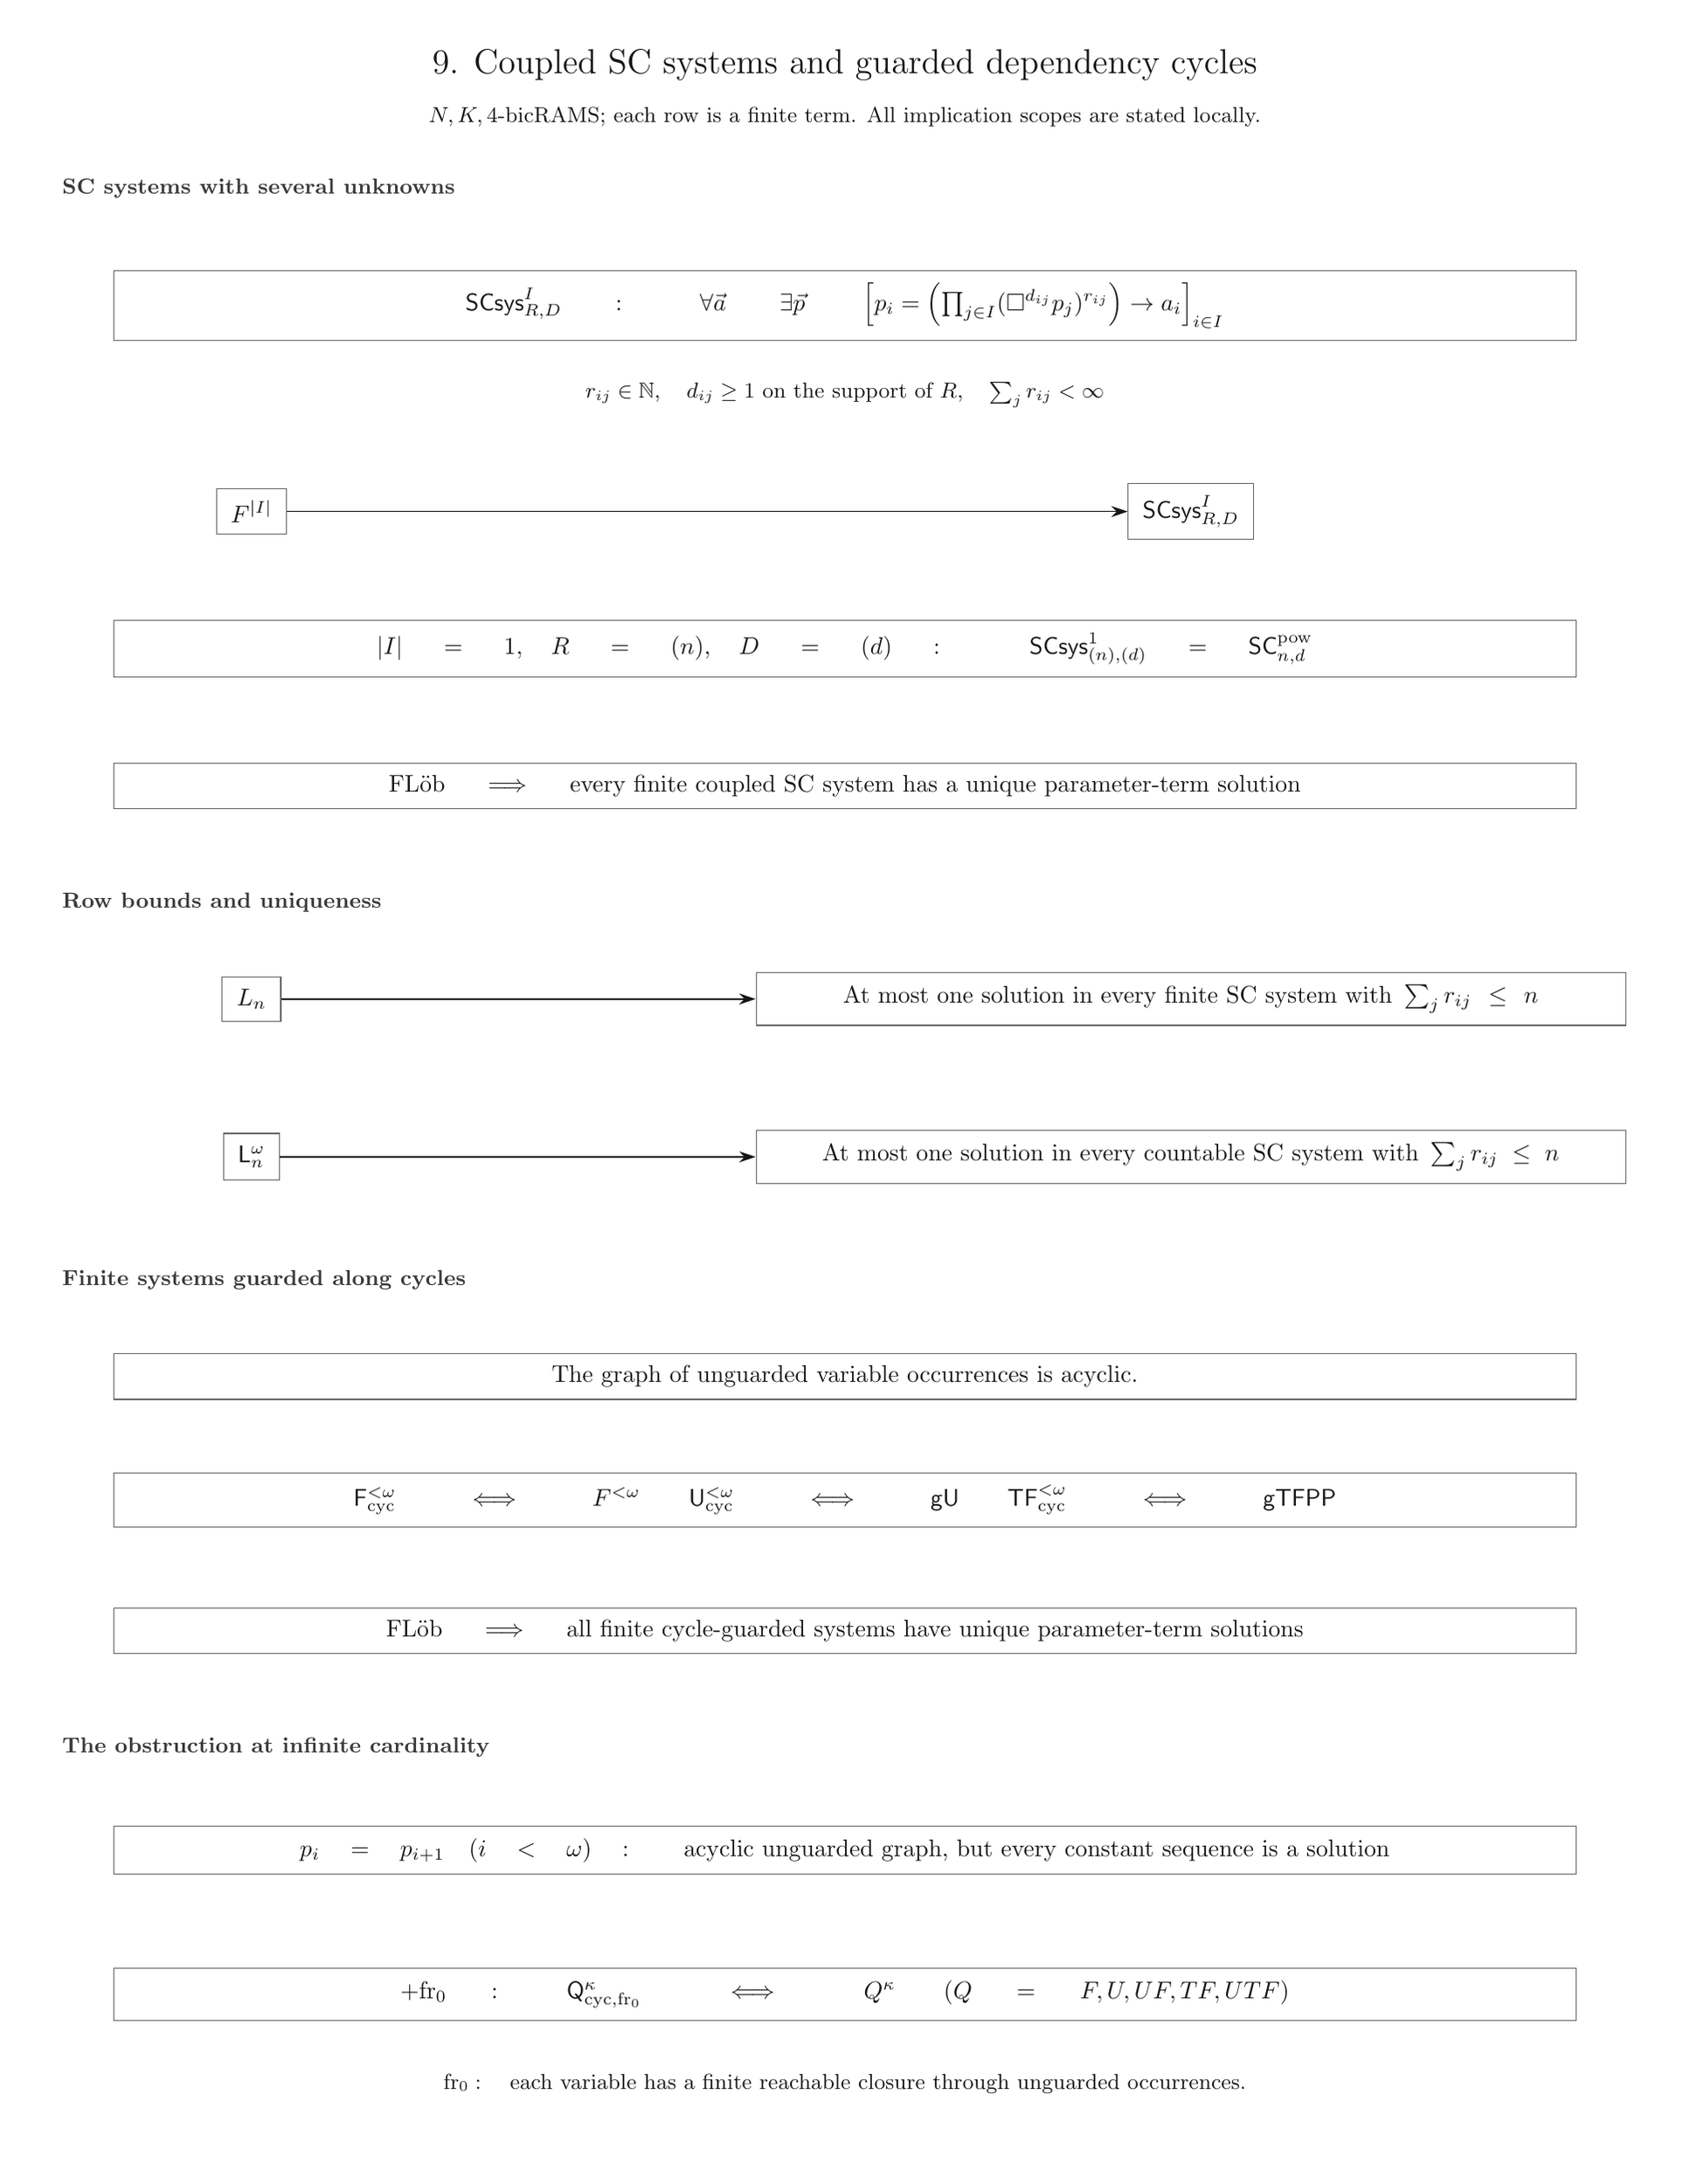
\begin{tikzpicture}[x=.72cm,y=1cm]
\path[use as bounding box] (-.6,-30) rectangle (32.6,1.1);
\Head{9. Coupled SC systems and guarded dependency cycles}{$N,K,4$-bicRAMS; each row is a finite term. All implication scopes are stated locally.}
\node[title] at (0,-1.3) {SC systems with several unknowns};
\node[p,text width=20.88cm] at (16,-3) {$\mathsf{SCsys}^{I}_{R,D}:\quad\forall\vec a\;\exists\vec p\;\left[p_i=\left(\prod_{j\in I}(\Box^{d_{ij}}p_j)^{r_{ij}}\right)\to a_i\right]_{i\in I}$};
\node[small] at (16,-4.3) {$r_{ij}\in\mathbb N,\quad d_{ij}\ge1\text{ on the support of }R,\quad\sum_jr_{ij}<\infty$};
\node[p] (gf) at (4,-6) {$F^{|I|}$};
\node[p] (scs) at (23,-6) {$\mathsf{SCsys}^{I}_{R,D}$};
\draw[arr] (gf)--(scs);
\node[p,text width=20.88cm] at (16,-8) {$|I|=1,\quad R=(n),\quad D=(d):\qquad\mathsf{SCsys}^{1}_{(n),(d)}=\mathsf{SC}^{\rm pow}_{n,d}$};
\node[p,text width=20.88cm] at (16,-10) {$\FL\Longrightarrow\text{every finite coupled SC system has a unique parameter-term solution}$};
\node[title] at (0,-11.7) {Row bounds and uniqueness};
\node[p] (ln) at (4,-13.1) {$L_n$};
\node[p,text width=12.24cm] (ufin) at (23,-13.1) {$\text{At most one solution in every finite SC system with }\sum_jr_{ij}\le n$};
\draw[arr] (ln)--(ufin);
\node[p] (lwn) at (4,-15.4) {$\mathsf L_n^\omega$};
\node[p,text width=12.24cm] (uinf) at (23,-15.4) {$\text{At most one solution in every countable SC system with }\sum_jr_{ij}\le n$};
\draw[arr] (lwn)--(uinf);
\node[title] at (0,-17.2) {Finite systems guarded along cycles};
\node[p,text width=20.88cm] at (16,-18.6) {$\text{The graph of unguarded variable occurrences is acyclic.}$};
\node[p,text width=20.88cm] at (16,-20.4) {$\mathsf F^{<\omega}_{\rm cyc}\iff F^{<\omega}\qquad\mathsf U^{<\omega}_{\rm cyc}\iff\gU\qquad\mathsf{TF}^{<\omega}_{\rm cyc}\iff\gT$};
\node[p,text width=20.88cm] at (16,-22.3) {$\FL\Longrightarrow\text{all finite cycle-guarded systems have unique parameter-term solutions}$};
\node[title] at (0,-24) {The obstruction at infinite cardinality};
\node[p,text width=20.88cm] at (16,-25.5) {$p_i=p_{i+1}\quad(i<\omega):\quad\text{acyclic unguarded graph, but every constant sequence is a solution}$};
\node[p,text width=20.88cm] at (16,-27.6) {$+\mathrm{fr}_0:\quad\mathsf Q^{\kappa}_{\rm cyc,fr_0}\iff Q^\kappa\qquad(Q=F,U,UF,TF,UTF)$};
\node[small] at (16,-28.9) {$\mathrm{fr}_0:\quad\text{each variable has a finite reachable closure through unguarded occurrences.}$};
\end{tikzpicture}
\end{document}
